\documentclass{ocbeameruni}


\setdefaultlanguage[babelshorthands=true]{german}


% Nur benötigt für die Beispiel-Listings!
\usepackage{listings}
\lstloadlanguages{[LaTeX]TeX}
\lstset{%
  basicstyle=\small \ttfamily,
  breaklines=true,
}

\newcommand{\R}{\mathbb{R}}


\title{Organic Computing 2}
\subtitle{Lösungsvorschlag Blatt07}
\date{\today}
\author{Lukas Huhn \and Qiang Chang \and Victor Gerling}
\institute{%
  Universität Augsburg\\
  Institut für Informatik\\
  Lehrstuhl für Organic Computing
}


\begin{document}


\maketitle


\begin{frame}{Gliederung}
  \setbeamertemplate{section in toc}[sections numbered]
  \tableofcontents
\end{frame}


\section{Aufgabe 02}

\begin{frame}{2.1 Einfache Binärkodierung}
Wie werden Lösungen binär kodiert? 
    \begin{itemize}
    \item Anhand des Wertebereichs und der Schrittweite wird ein unsigned integer generiert.
    \item Dieser wird mittels Integer.toBinaryString(i) (Java Funktion) in einen Binär-String umgewandelt.
    \item String wird evtl. mit zusäzlichen Nullen aufgefüllt, um gewünschte Stringlänge zu erreichen.
    \item Beispiel: siehe Code.
    \end{itemize}
\end{frame}

\begin{frame}{2.1 Einfache Binärkodierung}
Wie wird Population initialisiert? 
    \begin{itemize}
    \item Jeder Wert des Eingabe-Tupels wird zufällig anhand des Wertebereichs initialisiert.
    \end{itemize}
\end{frame}

\begin{frame}{2.1 Einfache Binärkodierung}
Wie werden Eltern ausgewählt? 
    \begin{itemize}
    \item Sortiere Population anhand des generierten Fitnesswertes.
    \item Erstelle so eine Rang-basierte Wahrscheinlichkeitsverteilung $\Rightarrow (1 - e^{- rank}) / (size population))$
    \item Ziehe mittels Roulette-Wheel Algortihmus n Eltern.
    \item Siehe Code.
    \end{itemize}
\end{frame}

\begin{frame}{2.1 Einfache Binärkodierung}
Wie wird Crossover durchgeführt? 
    \begin{itemize}
    \item Mittels uniform crossover.
    \item Entscheide bei jedem Bit zufällig, ob die Eltern ihr Bit vertauschen sollen.
    \item Siehe Code.
    \end{itemize}
\end{frame}

\begin{frame}{2.1 Einfache Binärkodierung}
Wie wird Mutation durchgeführt? 
    \begin{itemize}
    \item Setze Threshold für Mutation (0.05).
    \item Generiere bei jedem Bit Zufallszahl um zu entscheiden ob es zur Mutation kommt.
    \item Bitflip wenn Mutation.
    \item Siehe Code.
    \end{itemize}
\end{frame}

\begin{frame}{2.2 Graycode}
Wie wird Gray-Kodierung durchgeführt? 
    \begin{itemize}
    \item Encoding: n xor (n >> 1), z.B.: 2 xor (2 >> 1) $\Rightarrow 3 \Rightarrow (11)_2$
    \item Decoding: p := n; while(n >>= 1 != 0) do p := p xor n; return p;
    \item Siehe Code.
    \end{itemize}
\end{frame}


\section{Aufgabe 03}

\begin{frame}{3 GA mit Fließkommazahlen}
Implementieren Sie nun einen GA für die Blackboxen, der direkt auf den Fließkommazahlen-Vektoren
arbeitet! Nutzen Sie dabei ...
    \begin{itemize}
    \item Alles gleich wie A2 außer Mutation.
    \item Für Mutation: ziehe zufällige Zahl zwischen [-step, step] und addiere sie zum jeweiligen Wert hinzu!
    \end{itemize}
\end{frame}

\section{Aufgabe 04}

\begin{frame}{4 Auswertung}
Erwarten Sie, dass der GA mit Fließkommazahlen auf den Blackboxen besser oder schlechter
funktioniert? Warum?
    \begin{itemize}
    \item Erwartung: Nein.
    \item Das modifizieren der Bits erlaubt eine feingranulare Anpassung der Werte.
    \item Eventuell langsamer um zu konvergieren, zum Ende hin jedoch potentiell präziser!
    \end{itemize}
\end{frame}

\begin{frame}{4 Auswertung}
Entscheiden Sie sich bei jedem Verfahren für eine gute Parametrisierung und geben Sie diese,
die Stelle des auf diese Weise beim Testen gefundenen Optimums sowie dessen Wert an!
    \begin{itemize}
    \item GA simple: Population: 600-1000, Parents: 40-80, Mutation-Thres: 0.05, step-size: 0.01-1
    \item GA gray: gleich
    \item GA float: gleich bis auf Mutation; hier step-size: 0.01-5
    \end{itemize}
\end{frame}

\begin{frame}{4 Auswertung BB1}
    \begin{center}
    \begin{figure}
    \begin{tabular}{|c|c|c|c|} 
      \hline
      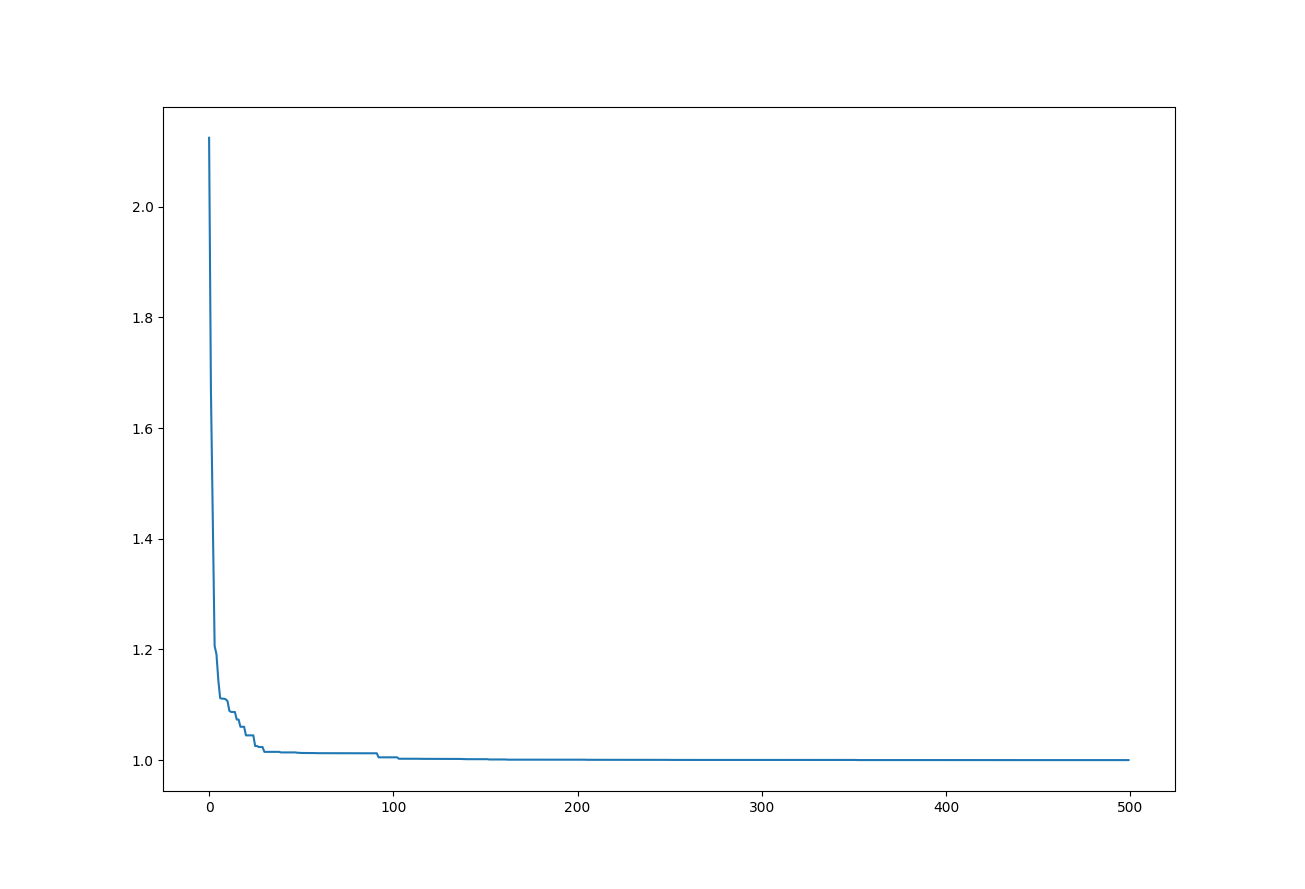
\includegraphics[width=23mm, height=20mm]{plots/bb1_naive.png} 
    & 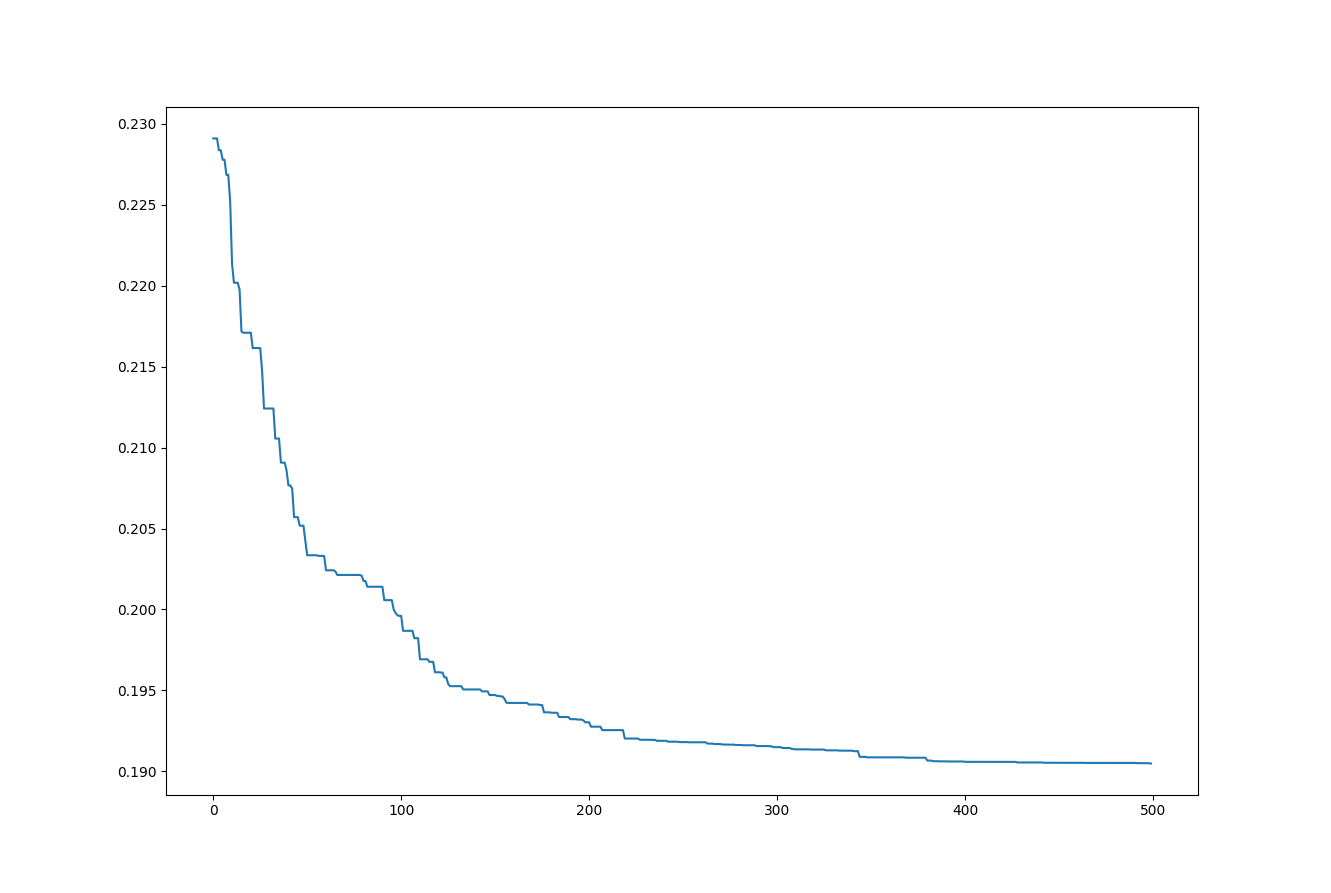
\includegraphics[width=23mm, height=20mm]{plots/bb1_ga_simple.png} 
    & 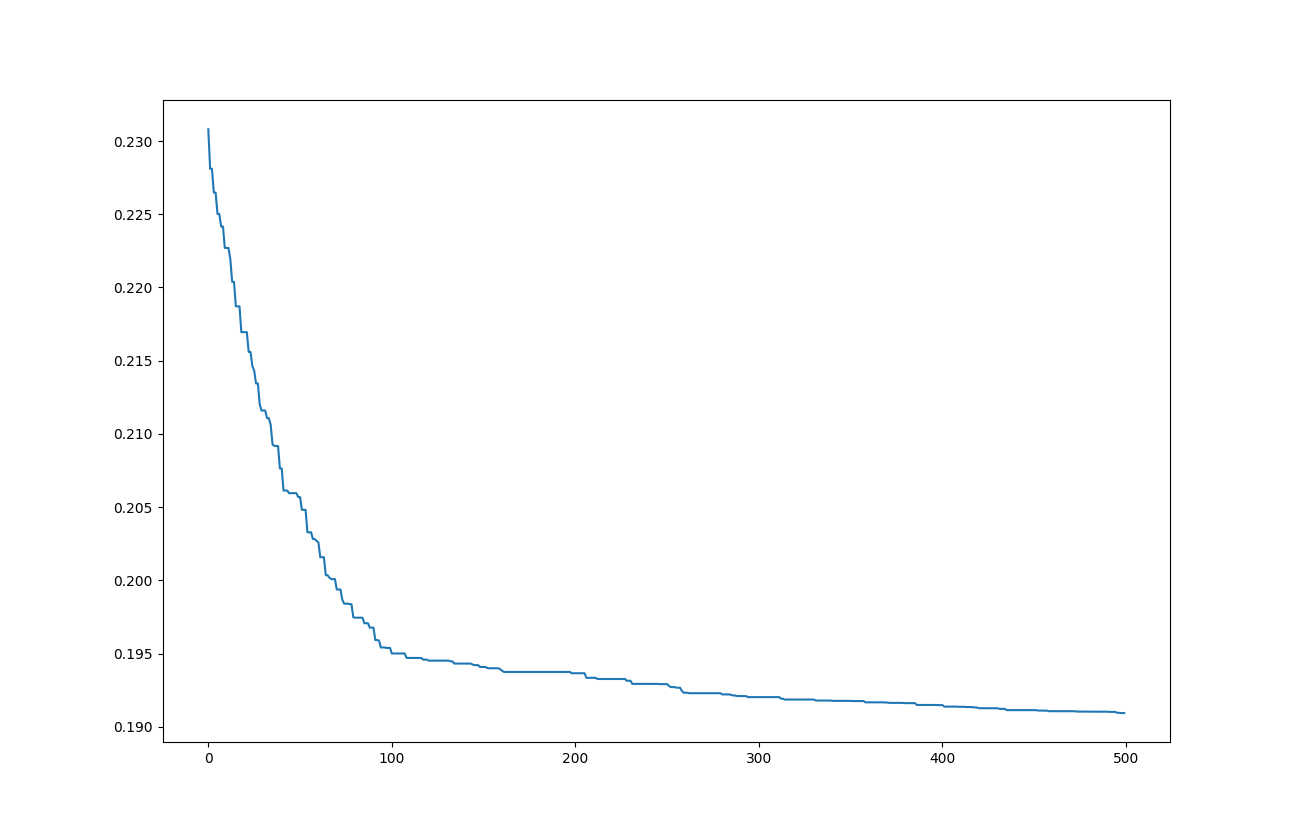
\includegraphics[width=23mm, height=20mm]{plots/bb1_ga_gray.png}
    & 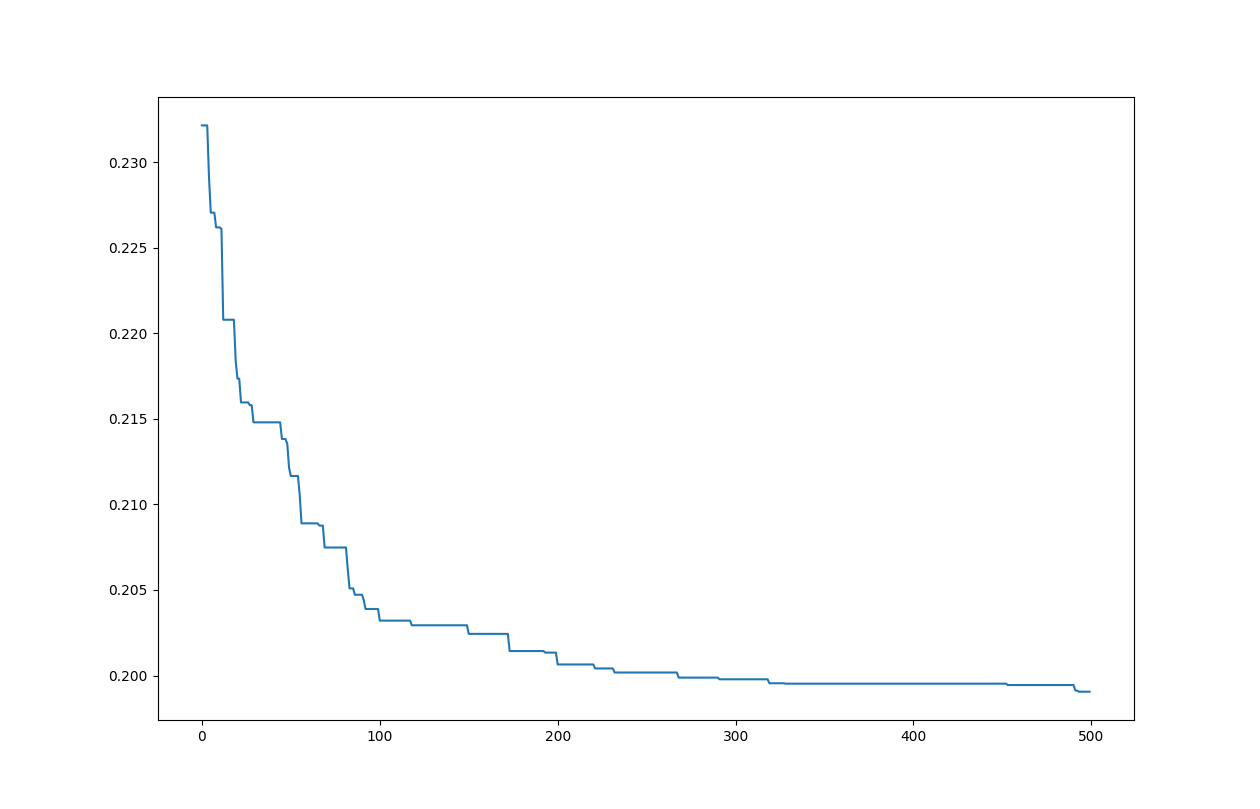
\includegraphics[width=23mm, height=20mm]{plots/bb1_ga_float.png} \\ \hline
      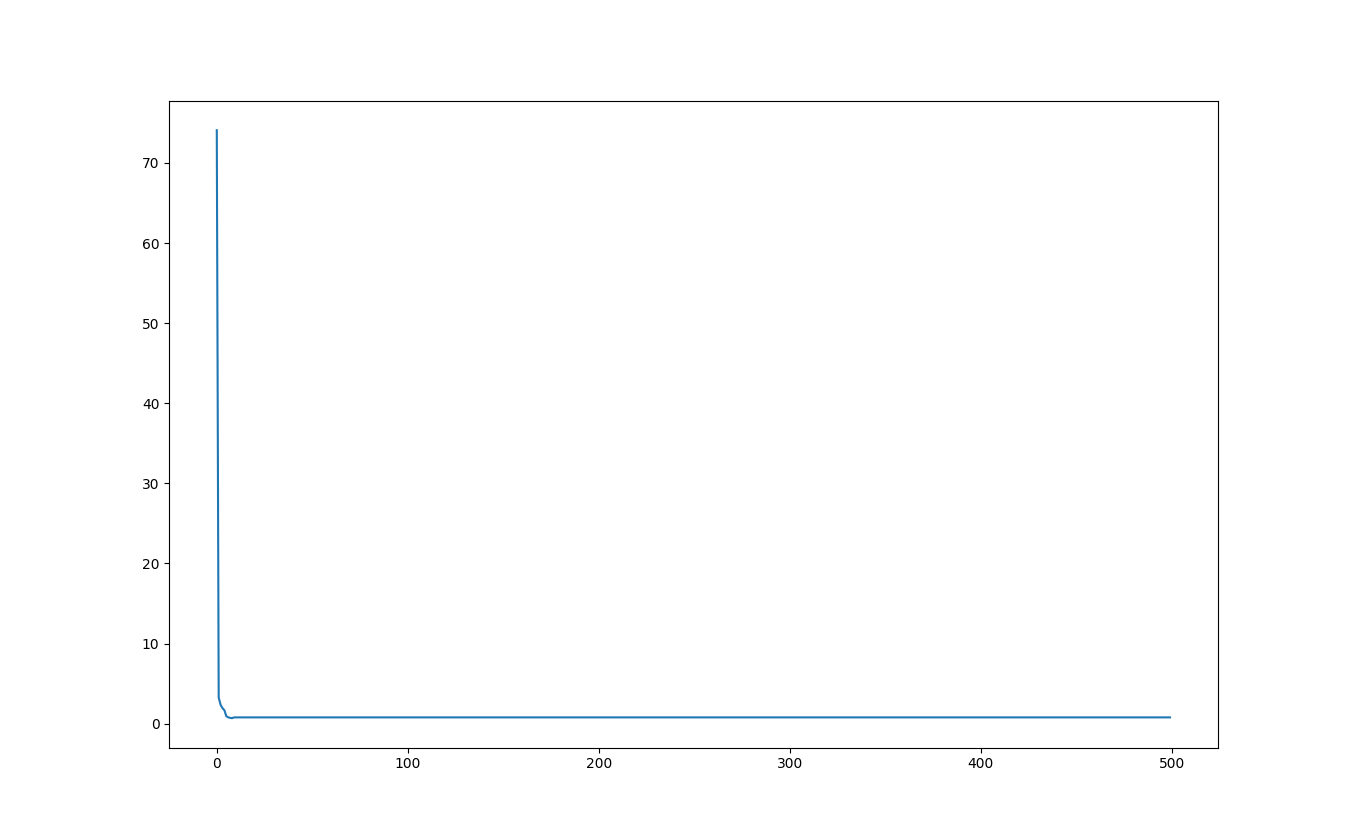
\includegraphics[width=23mm, height=20mm]{plots/bb1_hc.png} 
    & 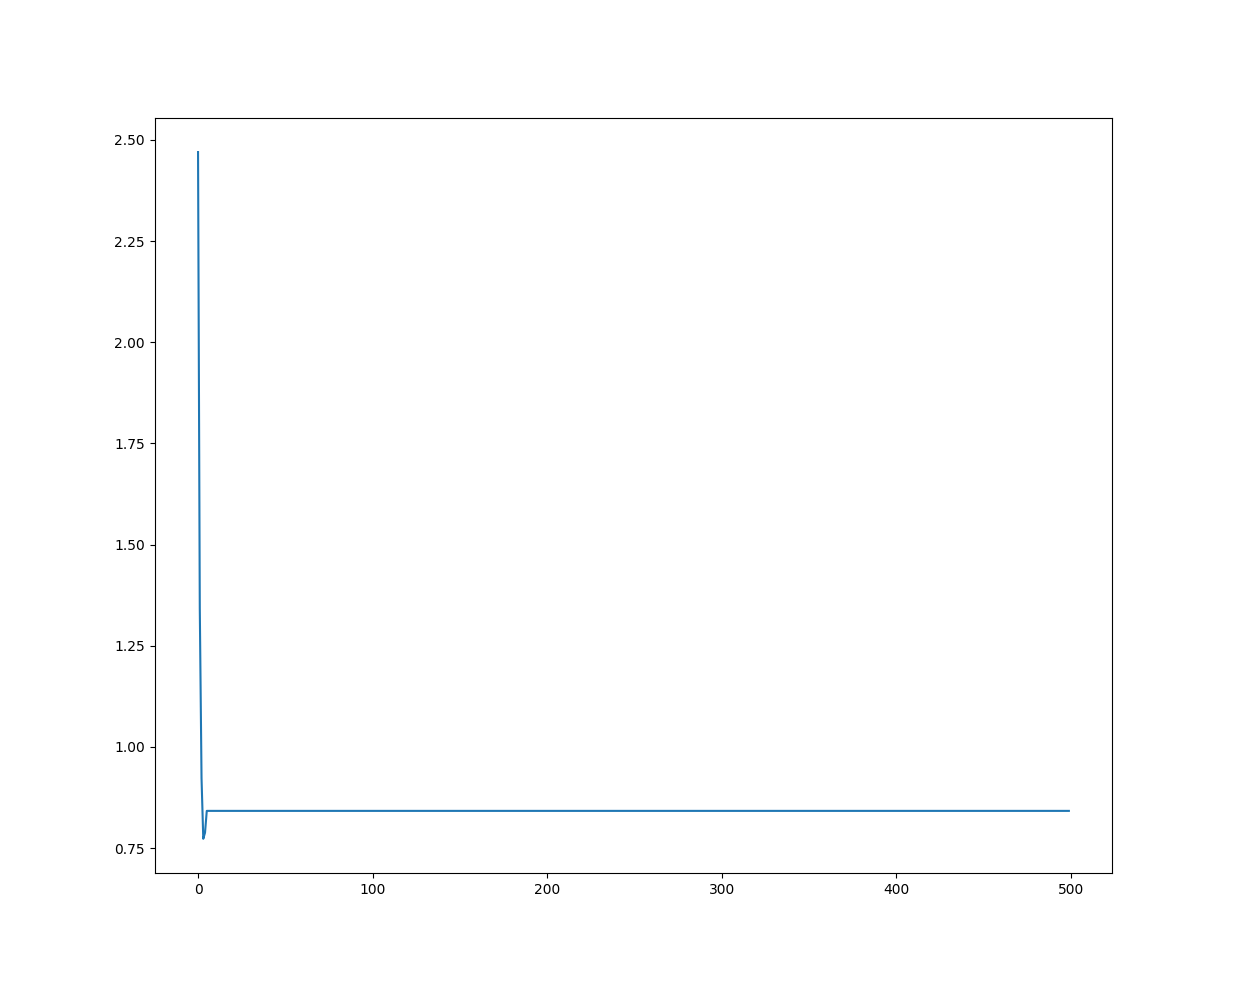
\includegraphics[width=23mm, height=20mm]{plots/bb1_hc_sa.png} 
    & 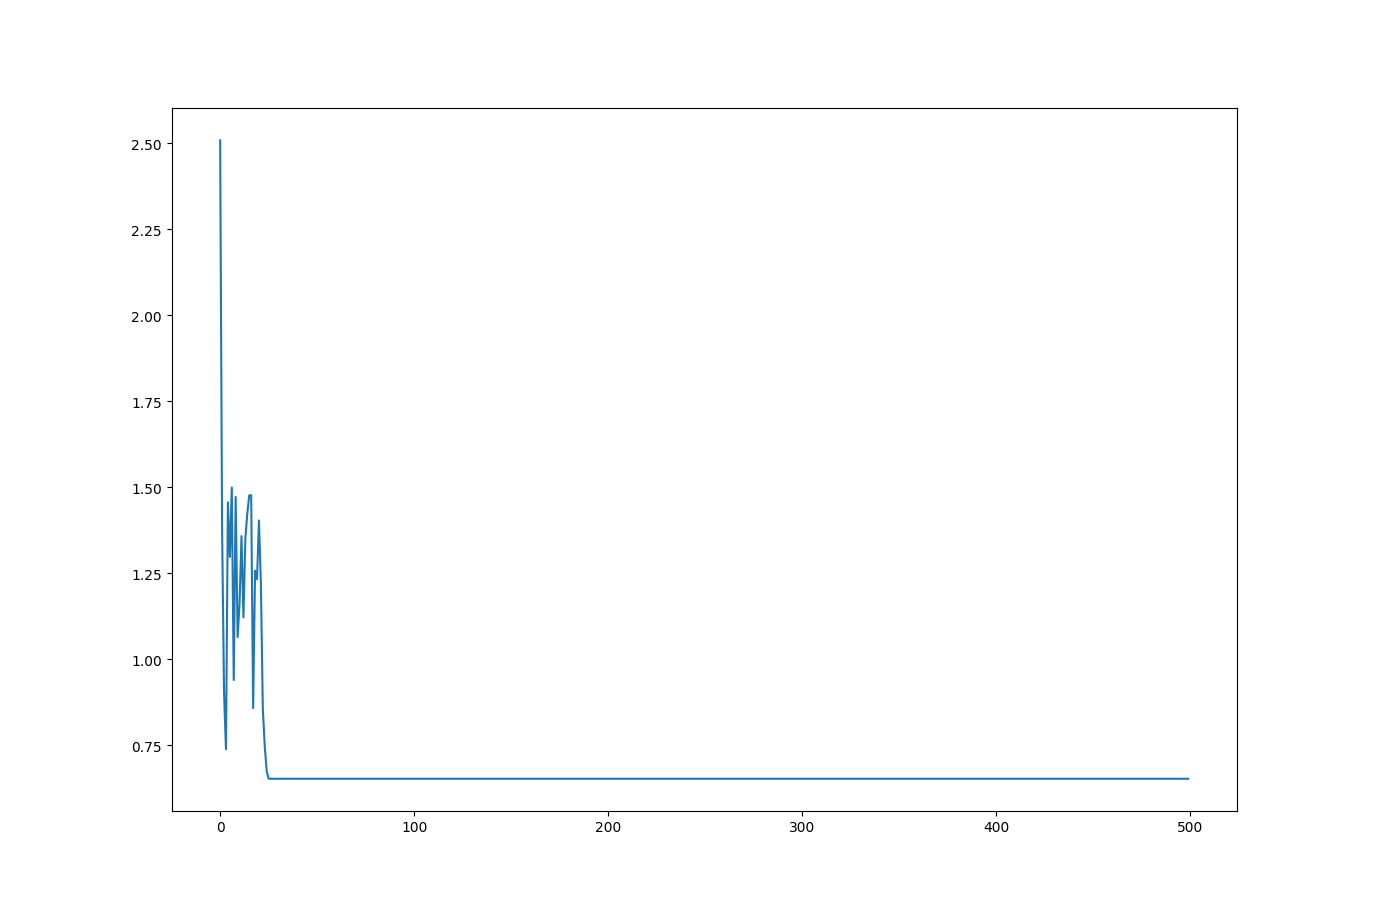
\includegraphics[width=23mm, height=20mm]{plots/bb1_hc_rs.png}
    & 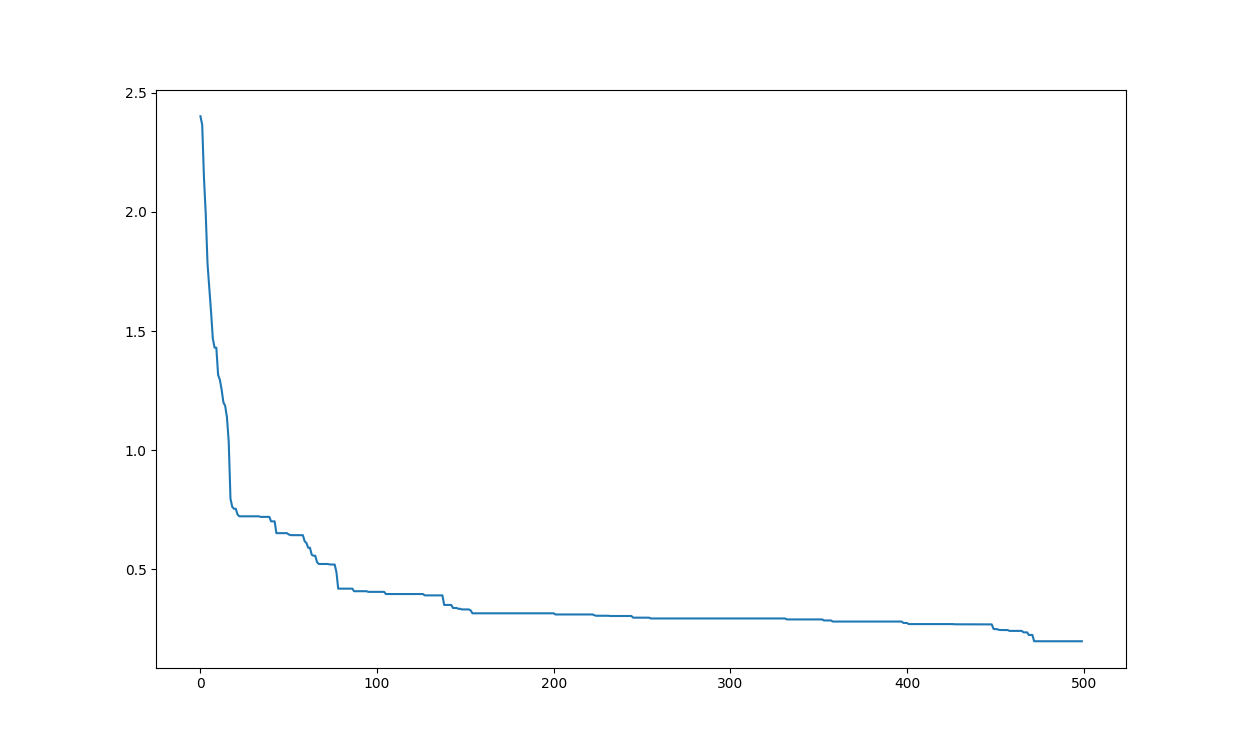
\includegraphics[width=23mm, height=20mm]{plots/bb1_sa.png} \\ \hline
    \end{tabular}
    \caption{Oben: Naives Verfahren, GA simple, GA gray, GA float \hspace{\textwidth}Unten: HC, HC steepest, HC random restart, simulated annealing}
    \end{figure}
    $\Rightarrow$ bestes Verfahren: ga-simple mit 100!
    \end{center}
\end{frame}

\begin{frame}{4 Auswertung BB2}
    \begin{center}
    \begin{figure}
    \begin{tabular}{|c|c|c|c|} 
      \hline
      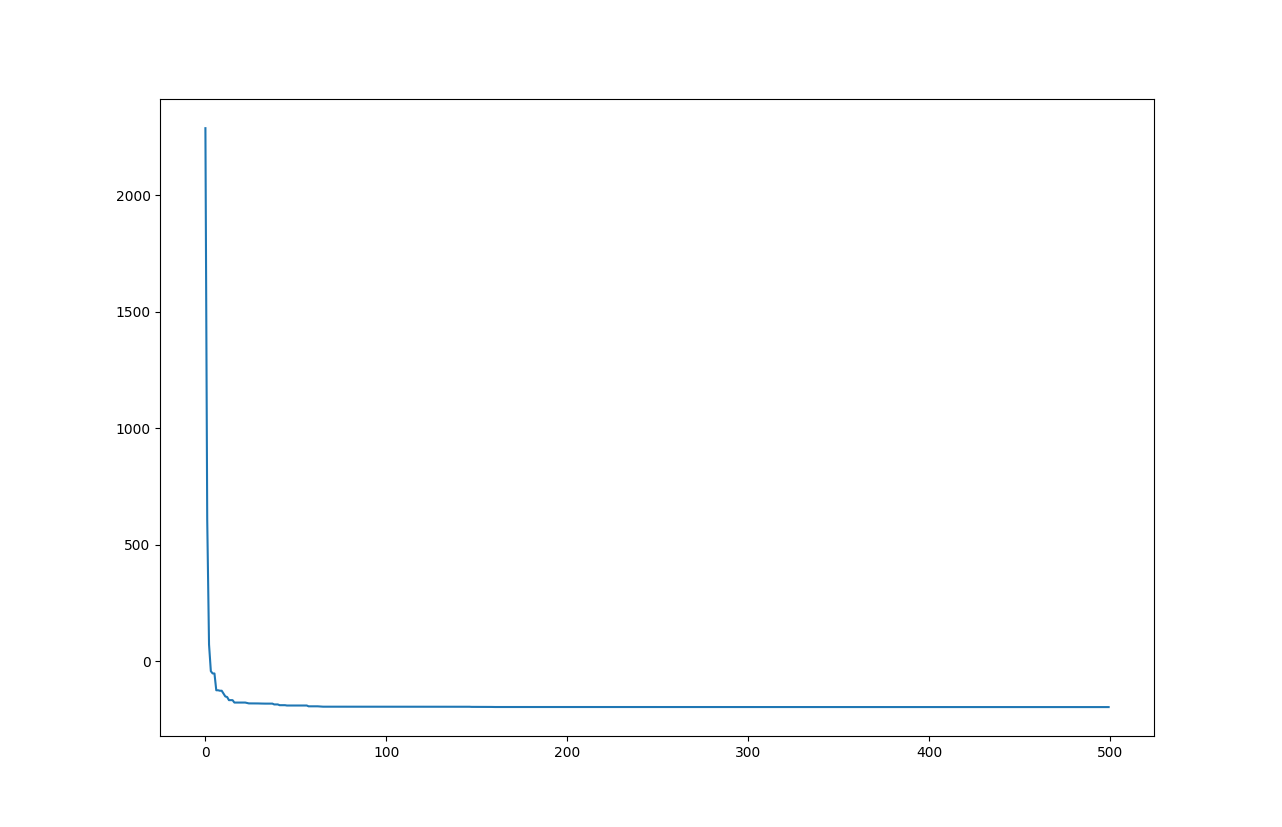
\includegraphics[width=23mm, height=20mm]{plots/bb2_naive.png} 
    & 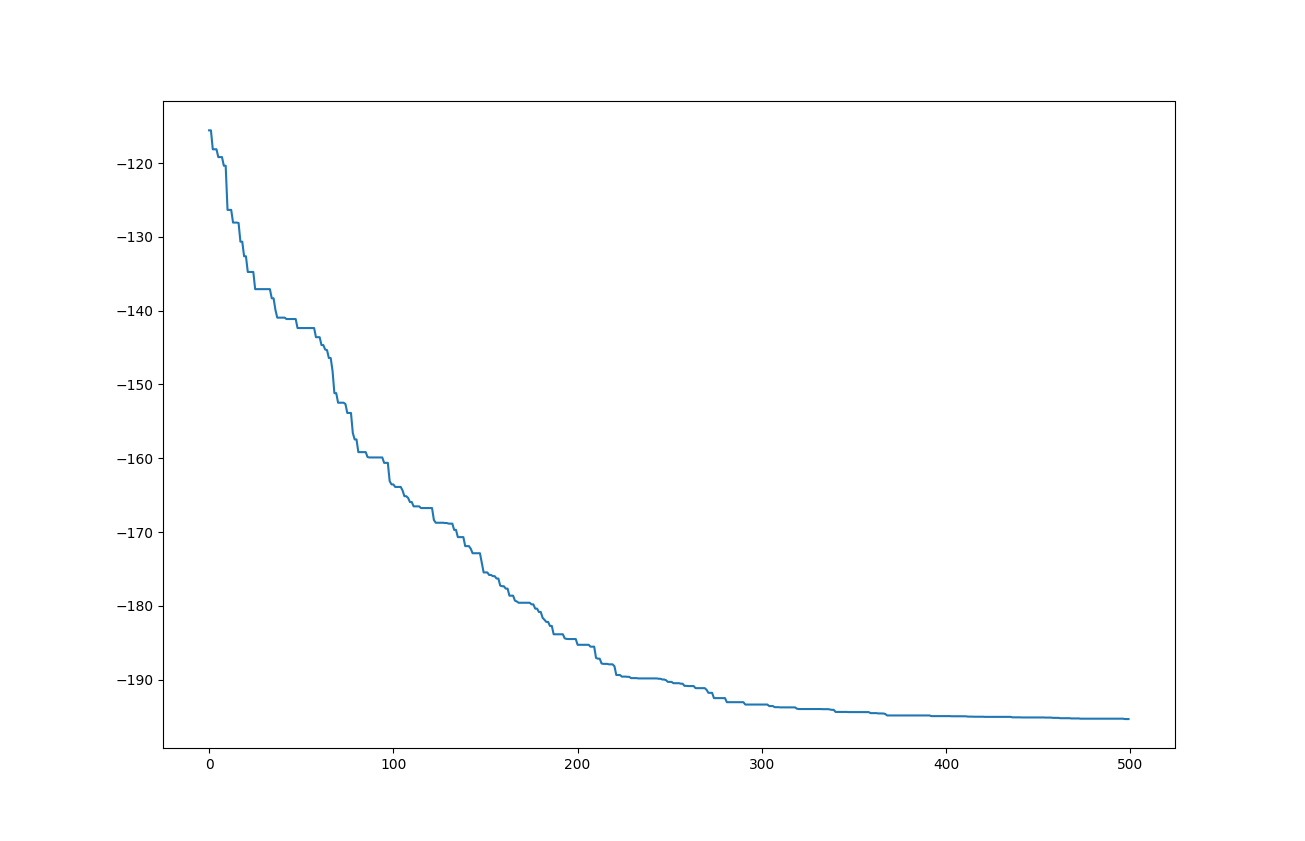
\includegraphics[width=23mm, height=20mm]{plots/bb2_ga_simple.png} 
    & 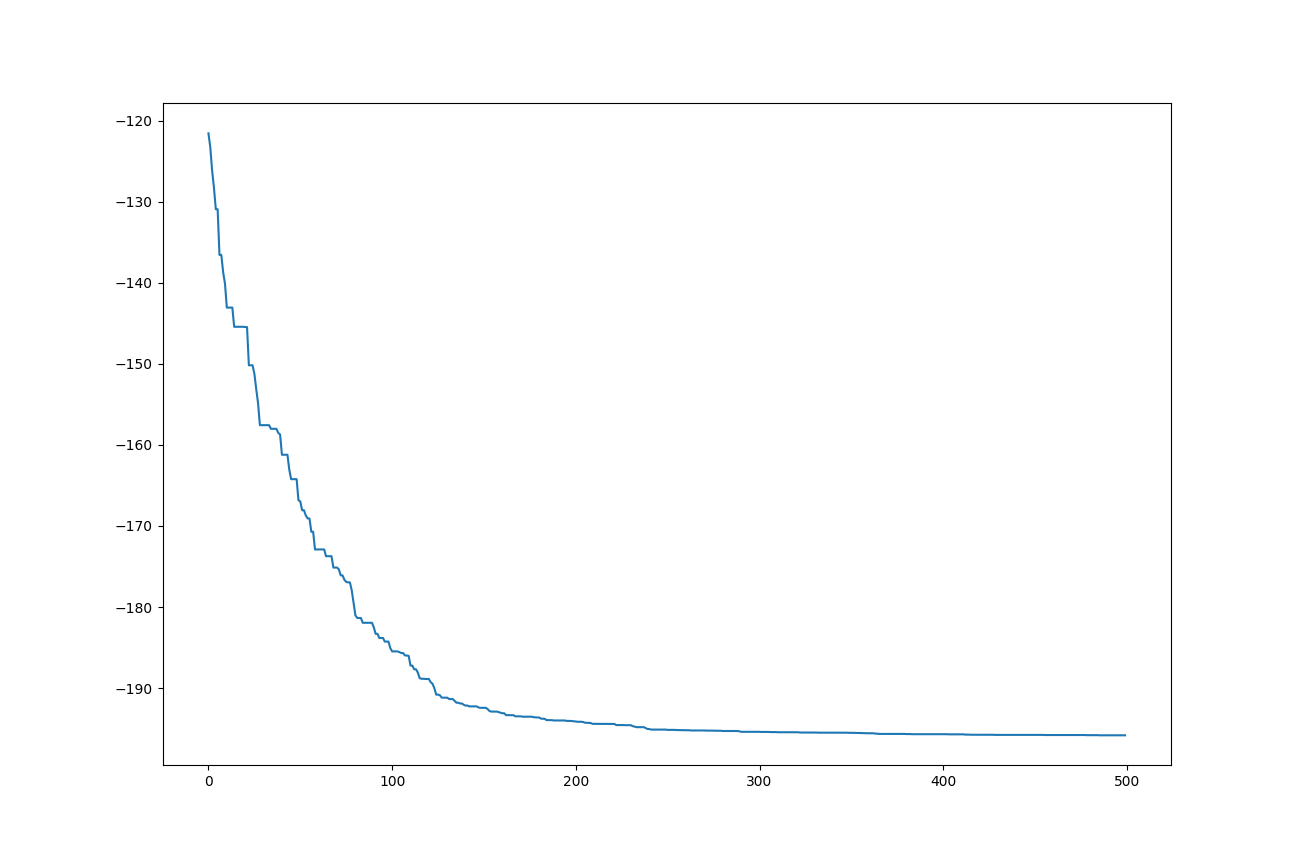
\includegraphics[width=23mm, height=20mm]{plots/bb2_ga_gray.png}
    & 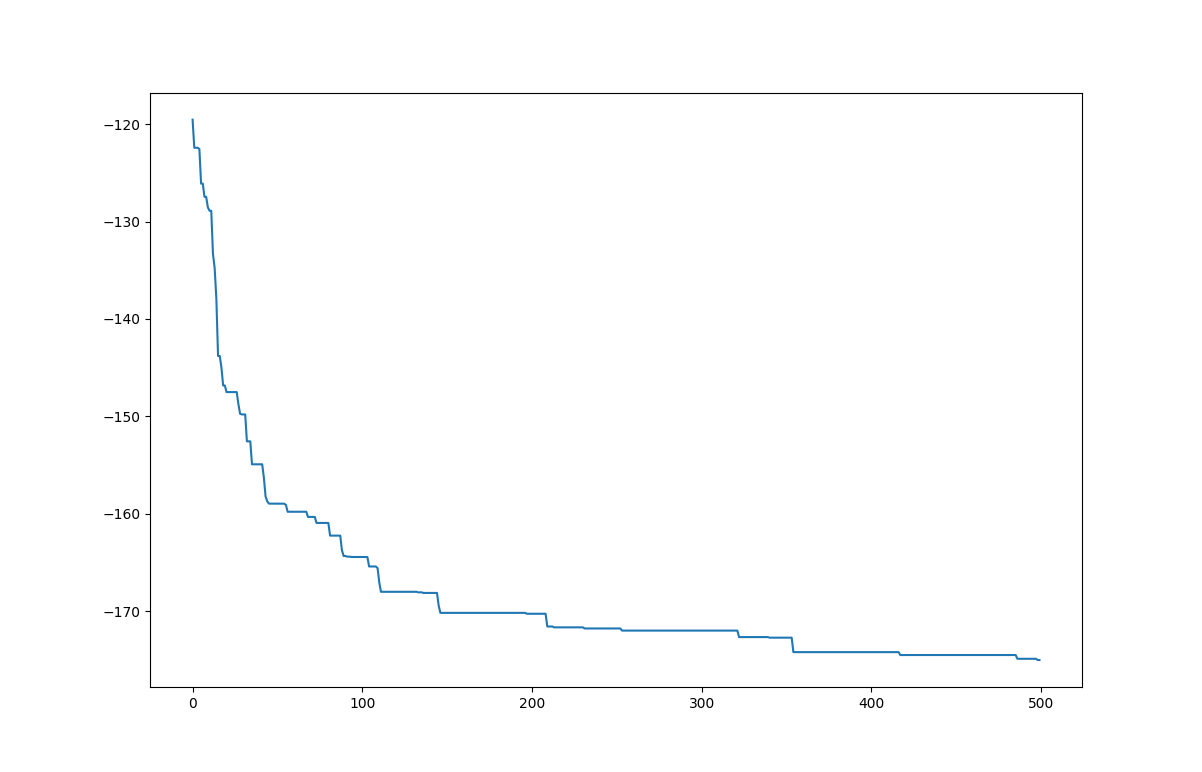
\includegraphics[width=23mm, height=20mm]{plots/bb2_ga_float.png} \\ \hline
      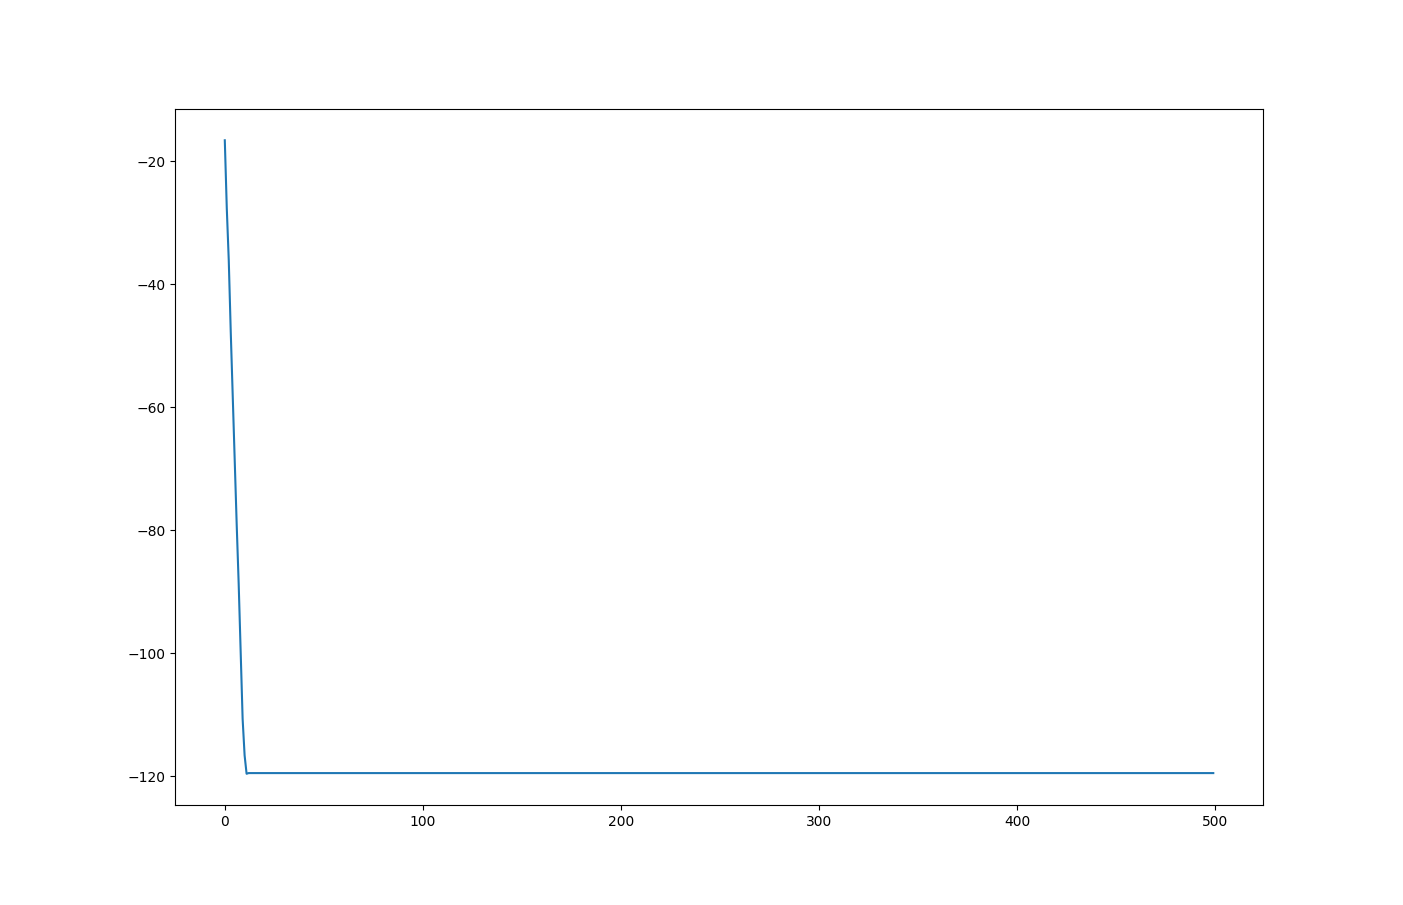
\includegraphics[width=23mm, height=20mm]{plots/bb2_hc.png} 
    & 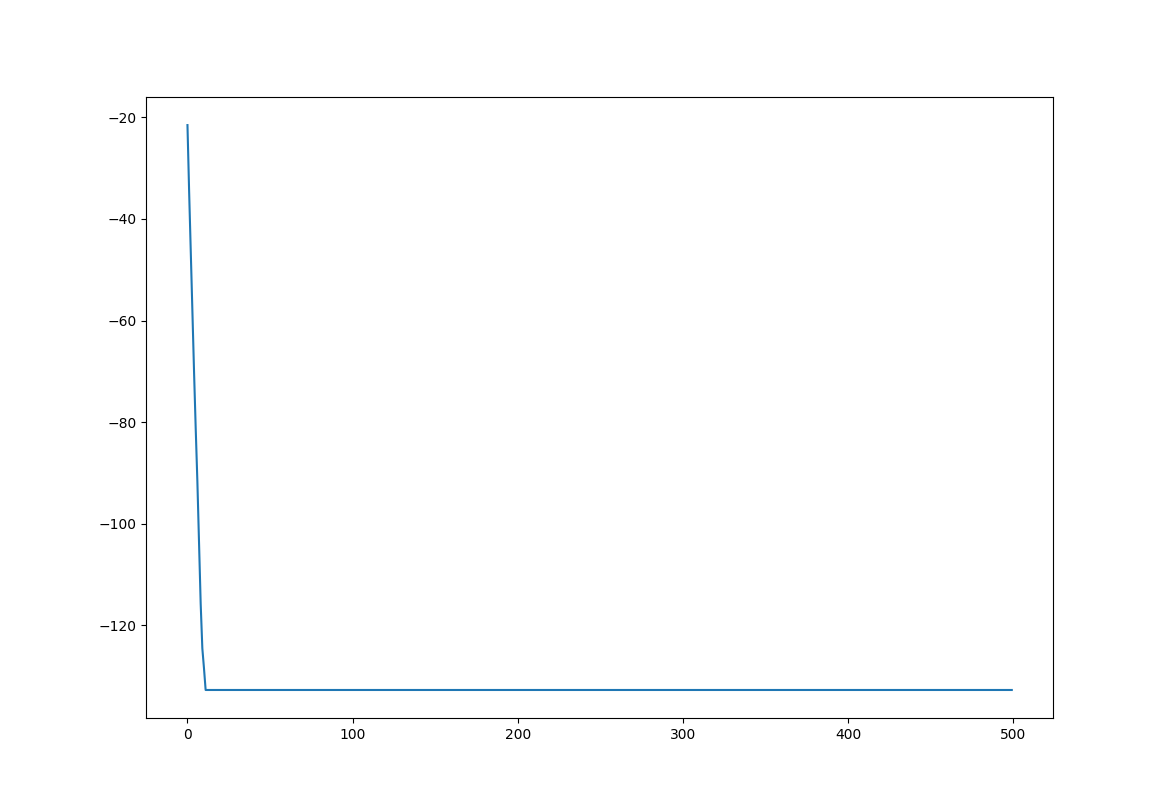
\includegraphics[width=23mm, height=20mm]{plots/bb2_hc_sa.png} 
    & 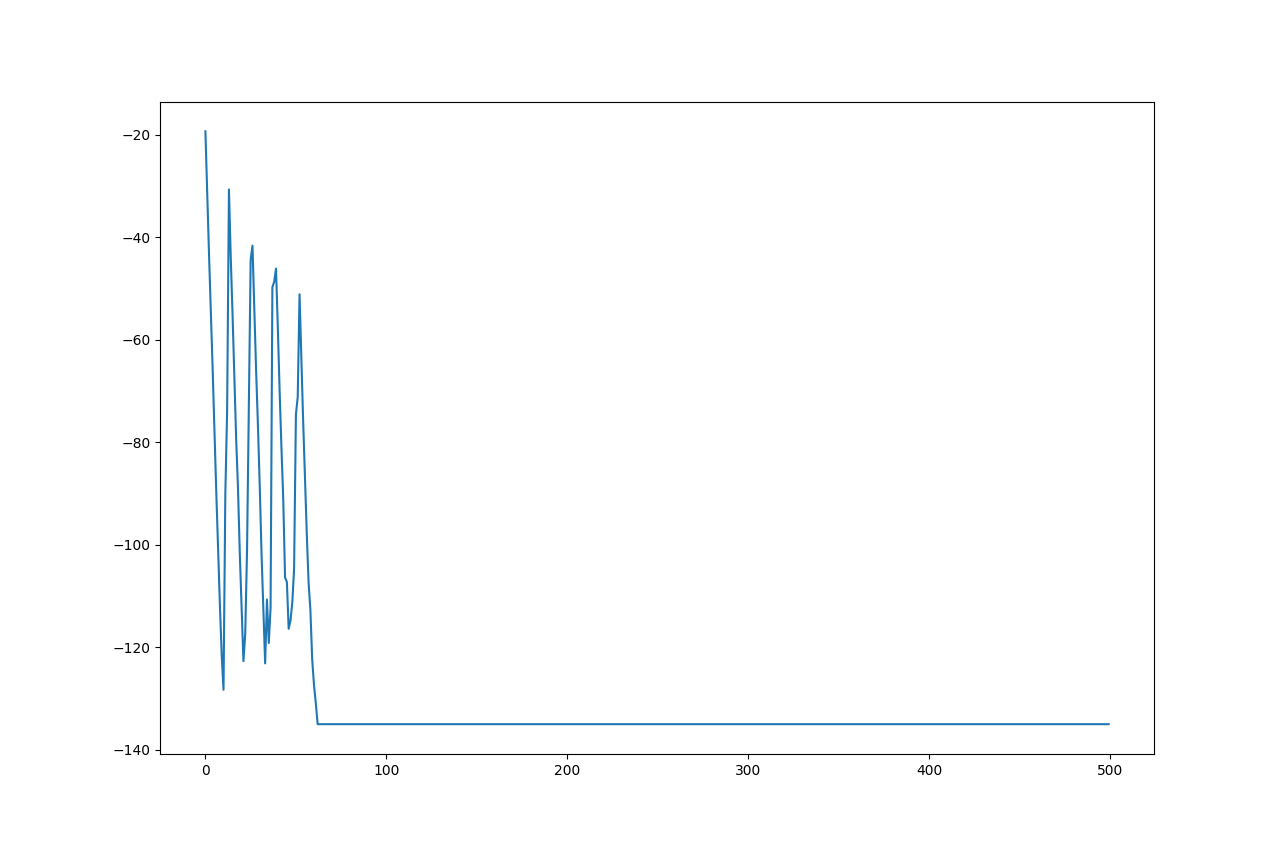
\includegraphics[width=23mm, height=20mm]{plots/bb2_hc_rs.png}
    & 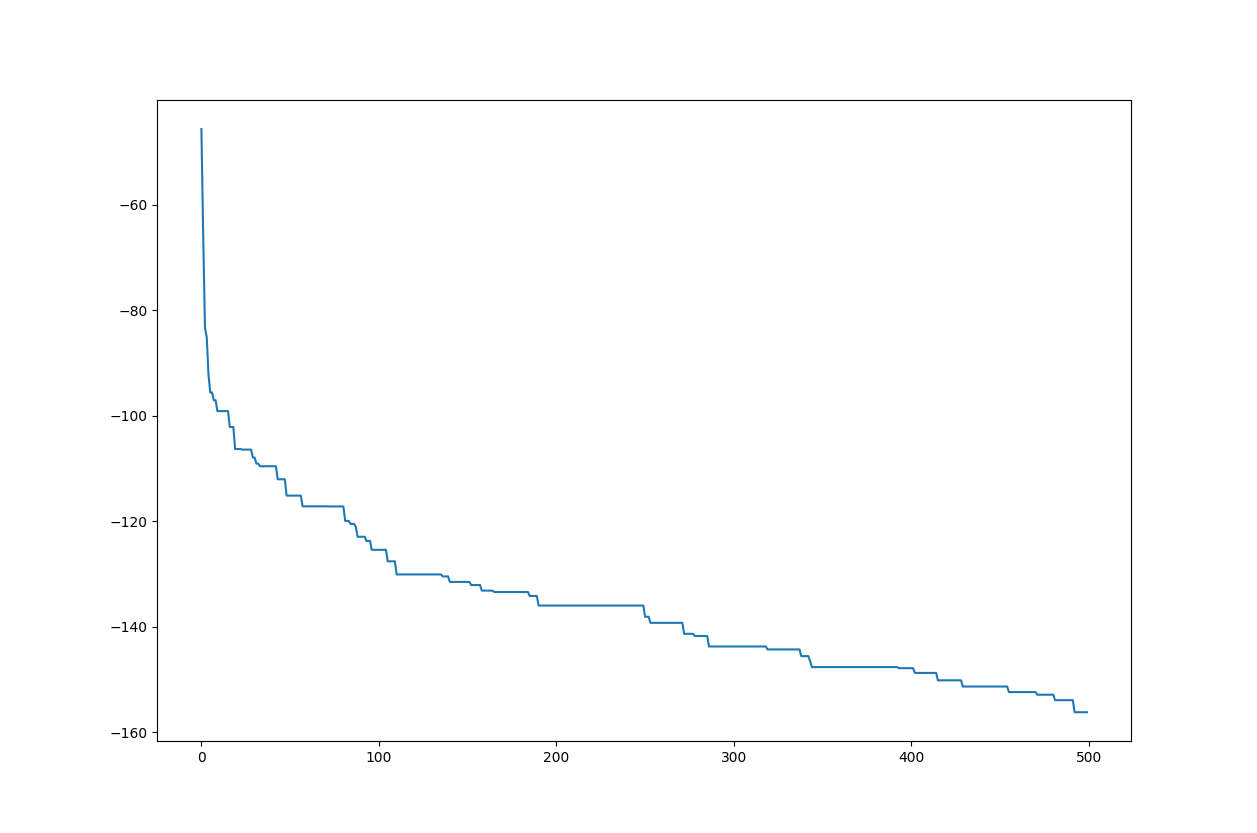
\includegraphics[width=23mm, height=20mm]{plots/bb2_sa.png} \\ \hline
    \end{tabular}
    \caption{Oben: Naives Verfahren, GA simple, GA gray, GA float \hspace{\textwidth}Unten: HC, HC steepest, HC random restart, simulated annealing}
    \end{figure}
    $\Rightarrow$ bestes Verfahren: ga-simple mit 100!
    \end{center}
\end{frame}

\begin{frame}{4 Auswertung BB3}
    \begin{center}
    \begin{figure}
    \begin{tabular}{|c|c|c|c|} 
      \hline
      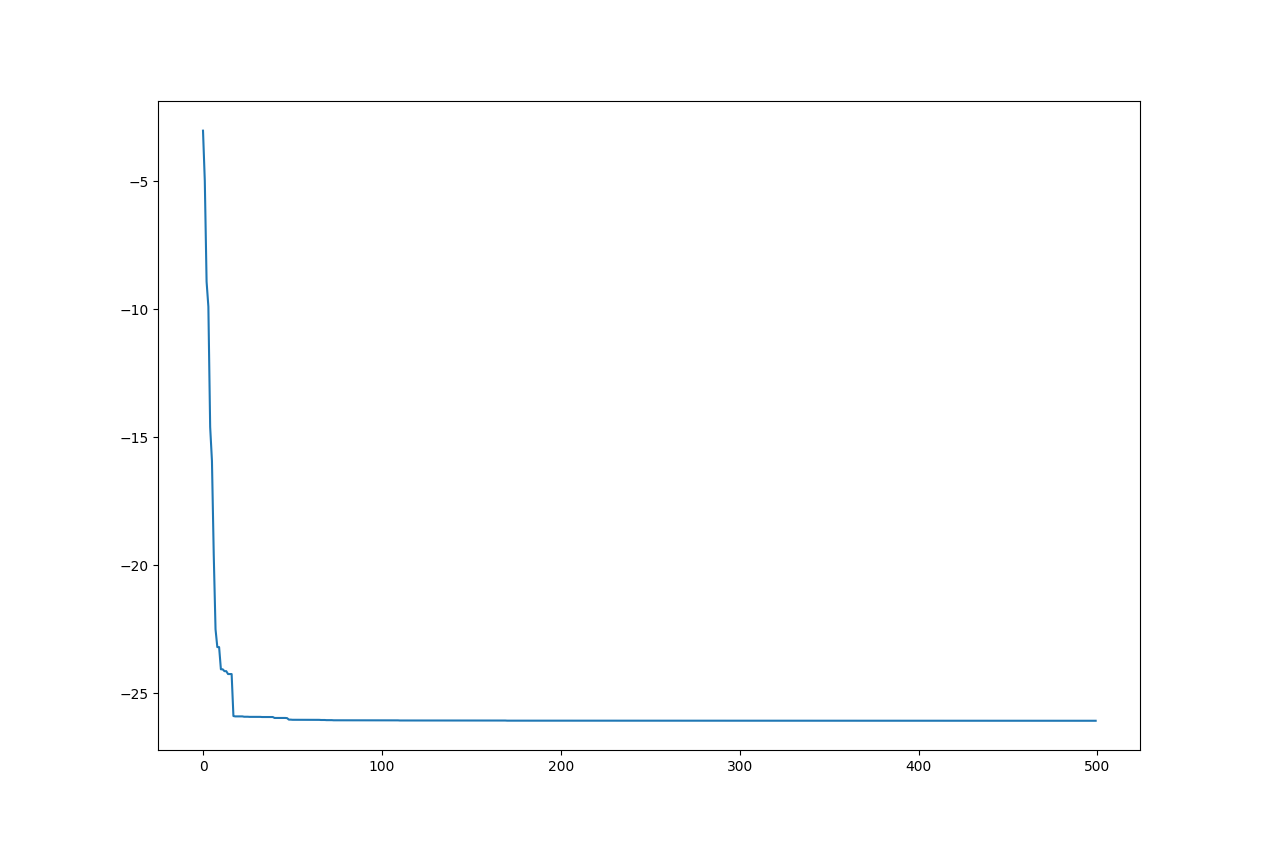
\includegraphics[width=23mm, height=20mm]{plots/bb3_naive.png} 
    & 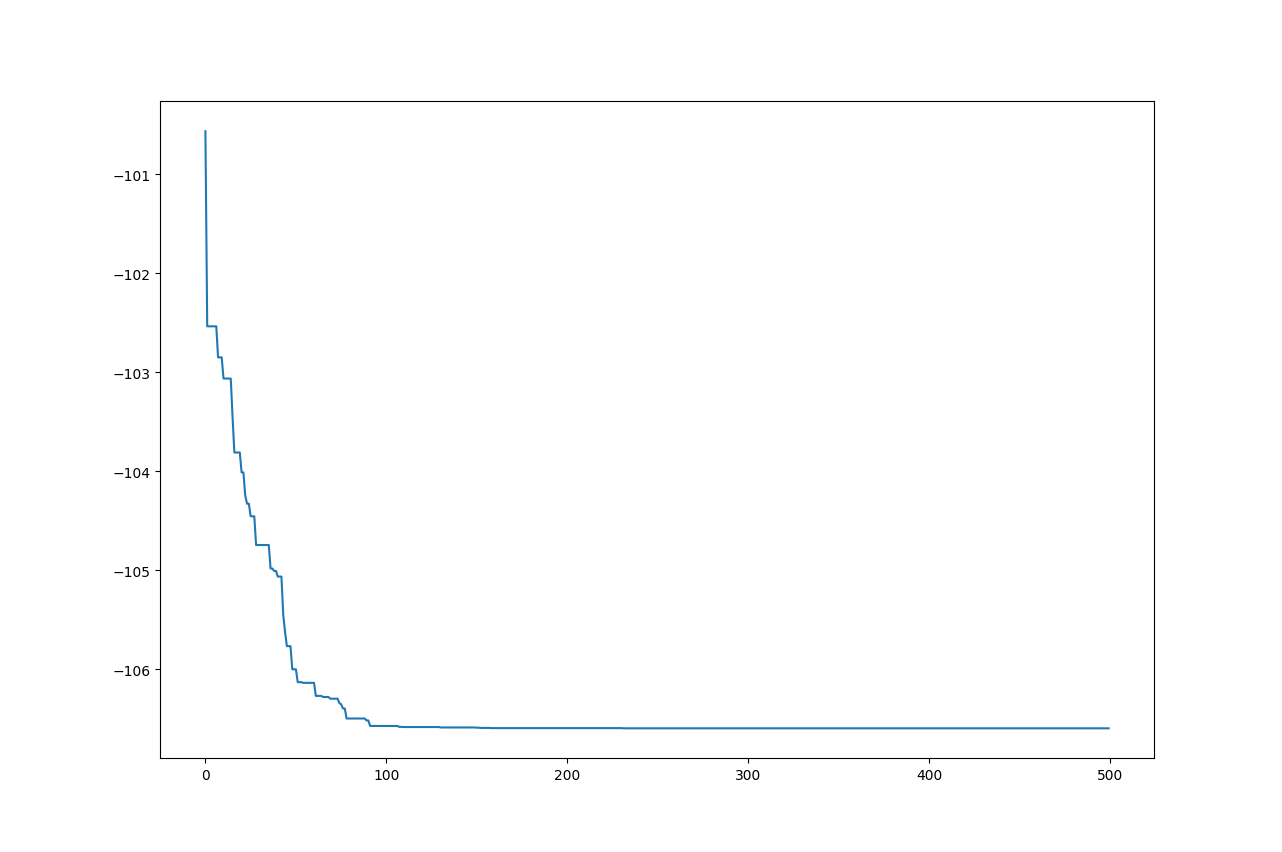
\includegraphics[width=23mm, height=20mm]{plots/bb3_ga_simple.png} 
    & 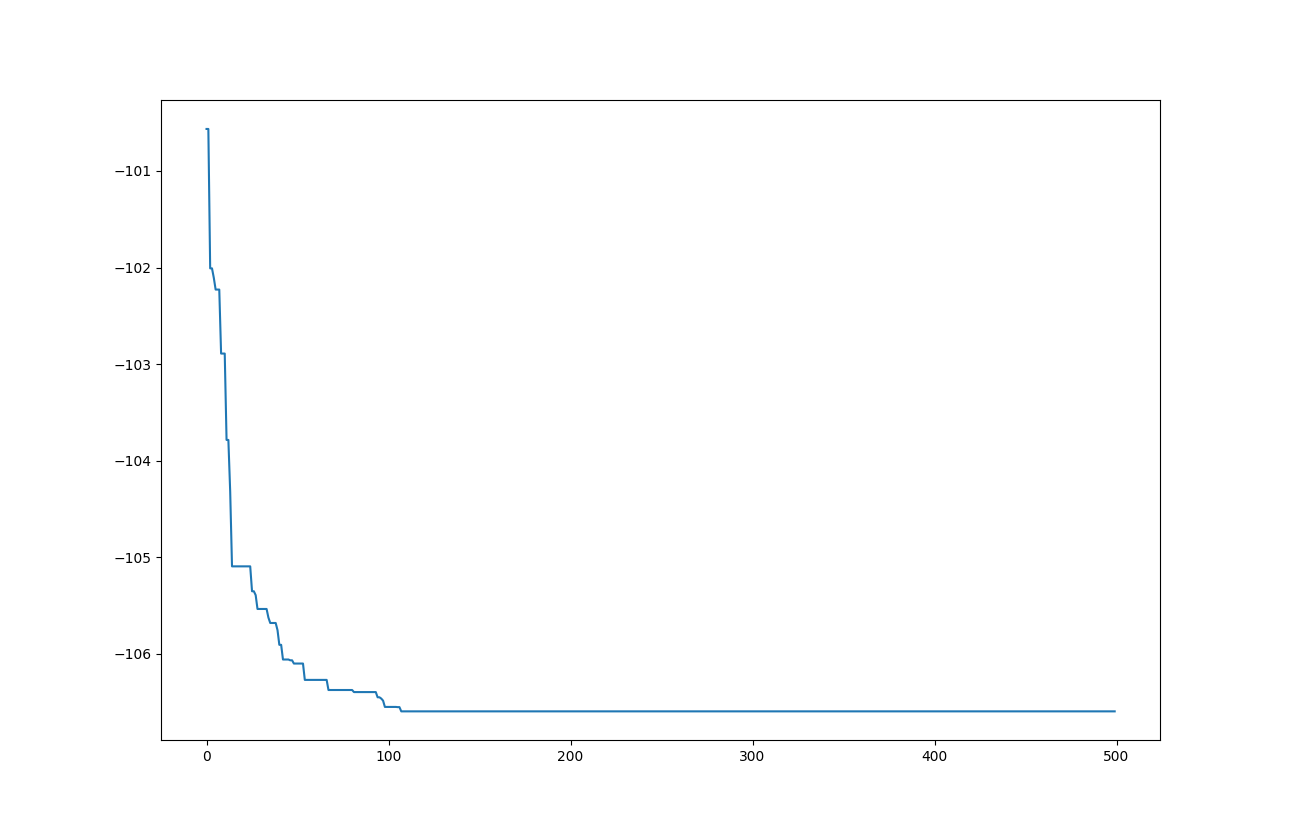
\includegraphics[width=23mm, height=20mm]{plots/bb3_ga_gray.png}
    & 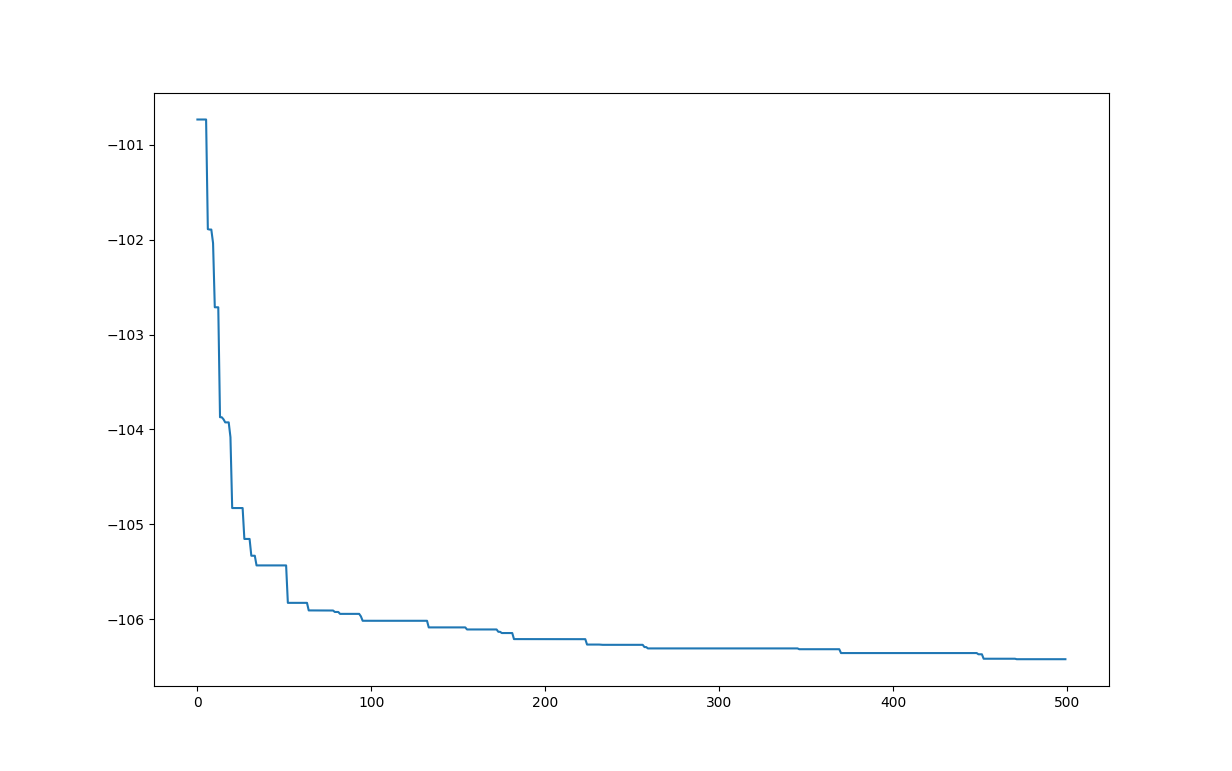
\includegraphics[width=23mm, height=20mm]{plots/bb3_ga_float.png} \\ \hline
      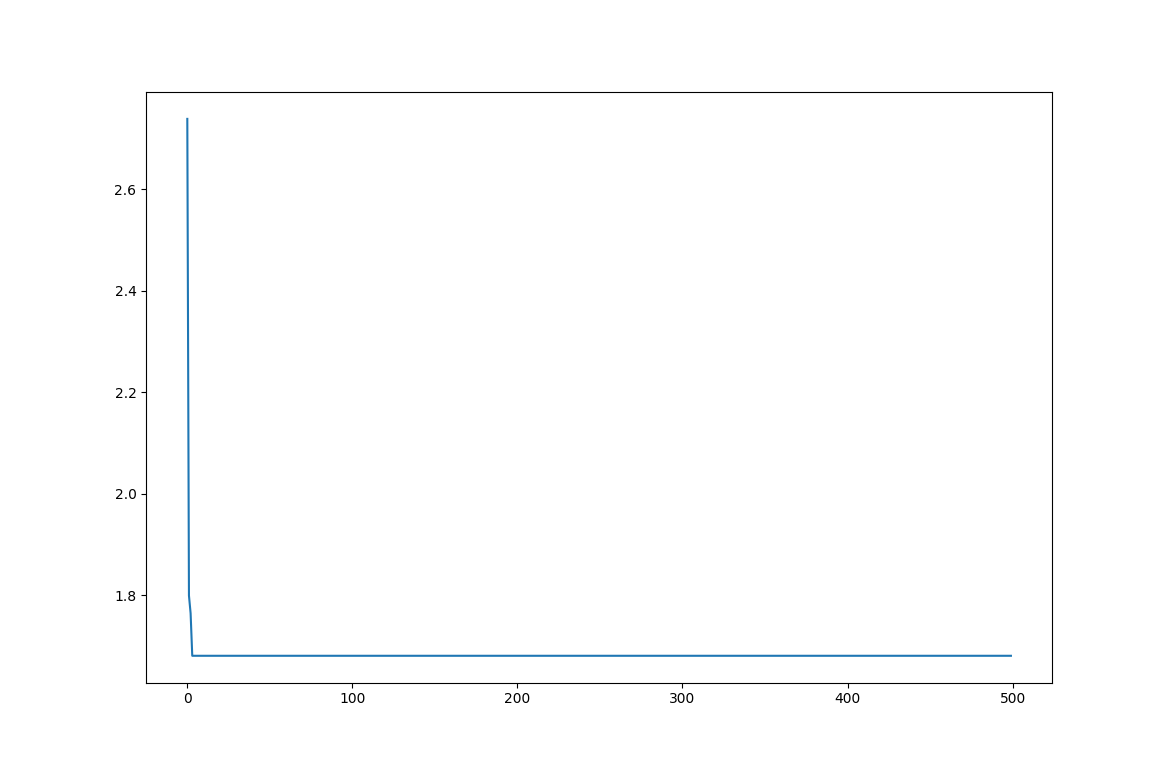
\includegraphics[width=23mm, height=20mm]{plots/bb3_hc.png} 
    & 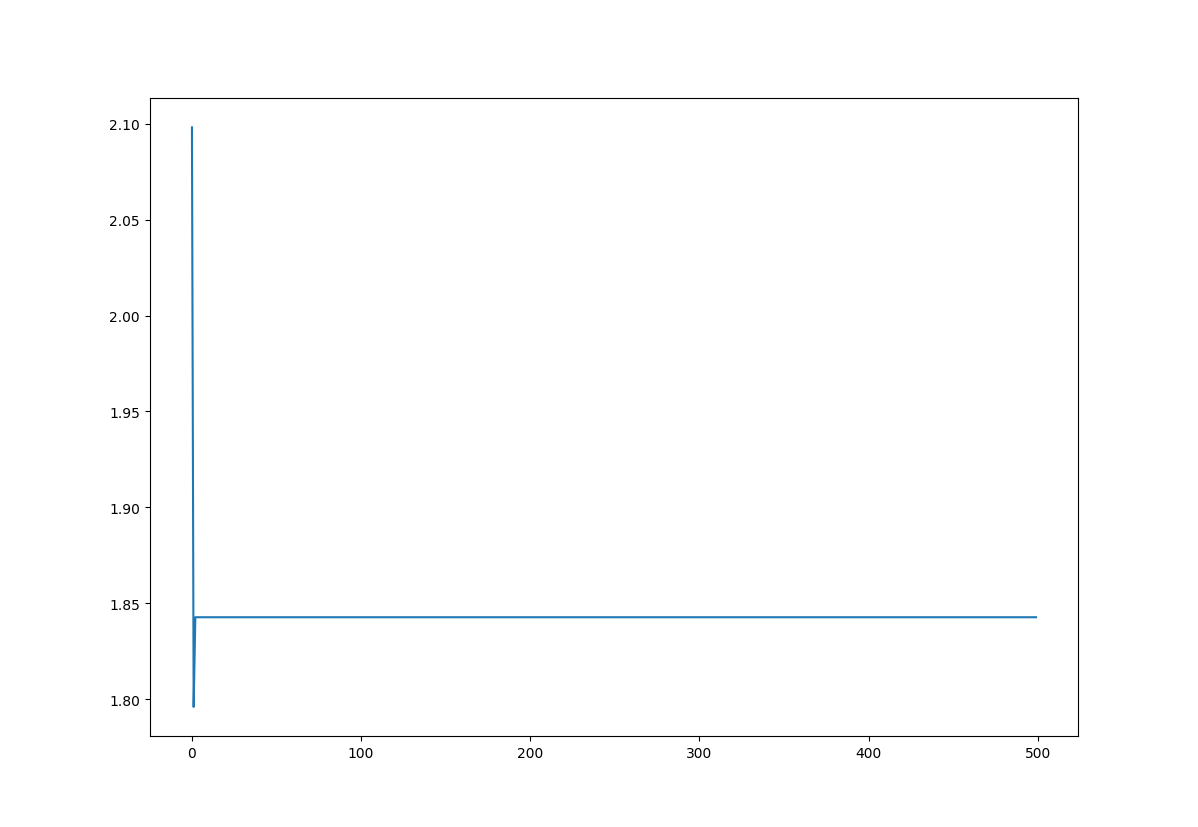
\includegraphics[width=23mm, height=20mm]{plots/bb3_hc_sa.png} 
    & 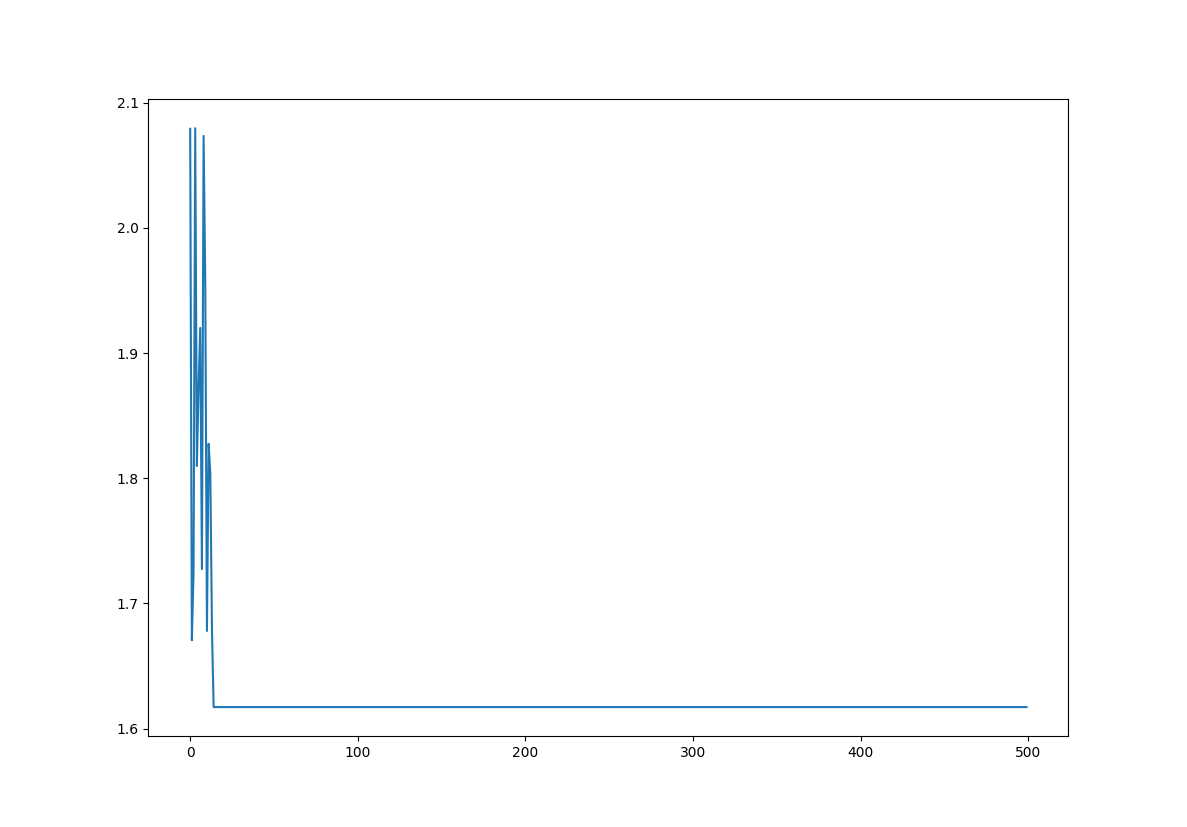
\includegraphics[width=23mm, height=20mm]{plots/bb3_hc_rs.png}
    & 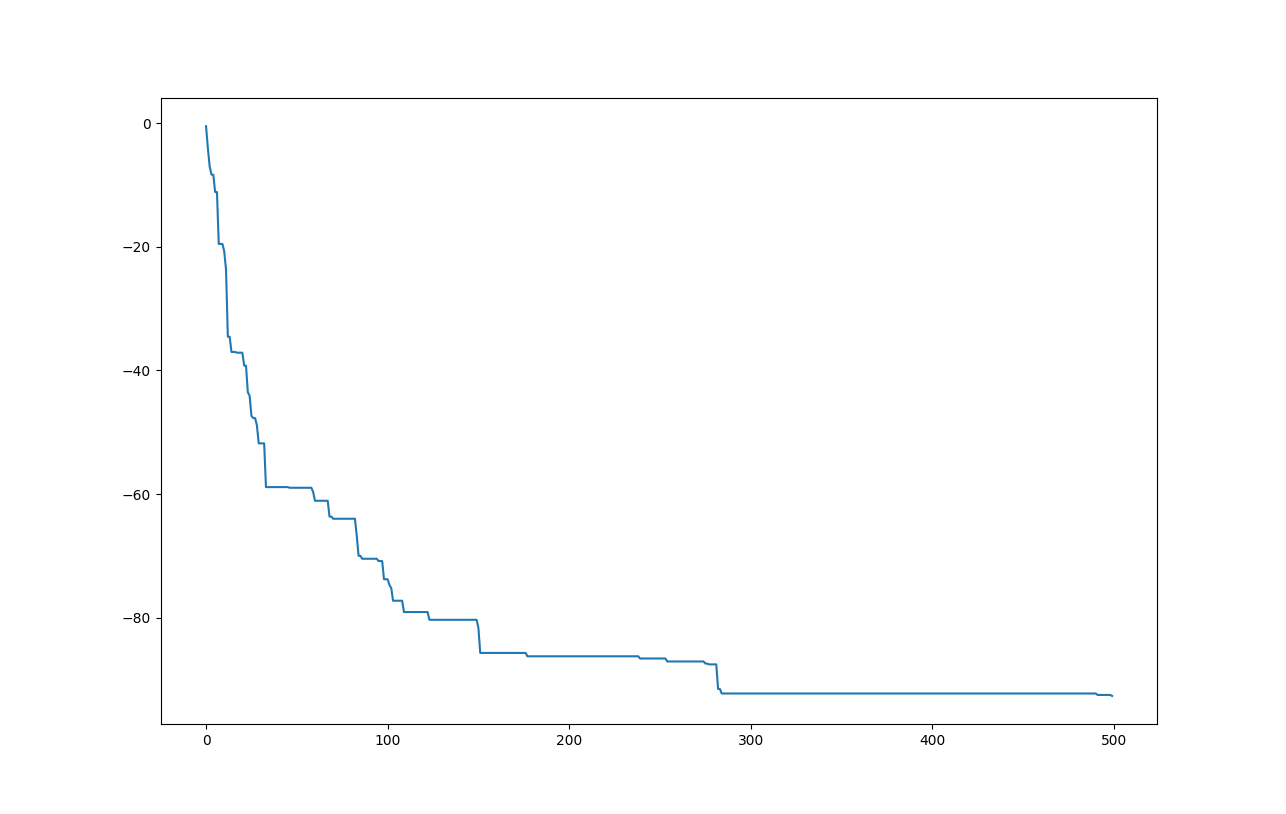
\includegraphics[width=23mm, height=20mm]{plots/bb3_sa.png} \\ \hline
    \end{tabular}
    \caption{Oben: Naives Verfahren, GA simple, GA gray, GA float \hspace{\textwidth}Unten: HC, HC steepest, HC random restart, simulated annealing}
    \end{figure}
    $\Rightarrow$ bestes Verfahren: ga-simple mit 100!
    \end{center}
\end{frame}

\begin{frame}{4 Auswertung BB4}
    \begin{center}
    \begin{figure}
    \begin{tabular}{|c|c|c|c|} 
      \hline
      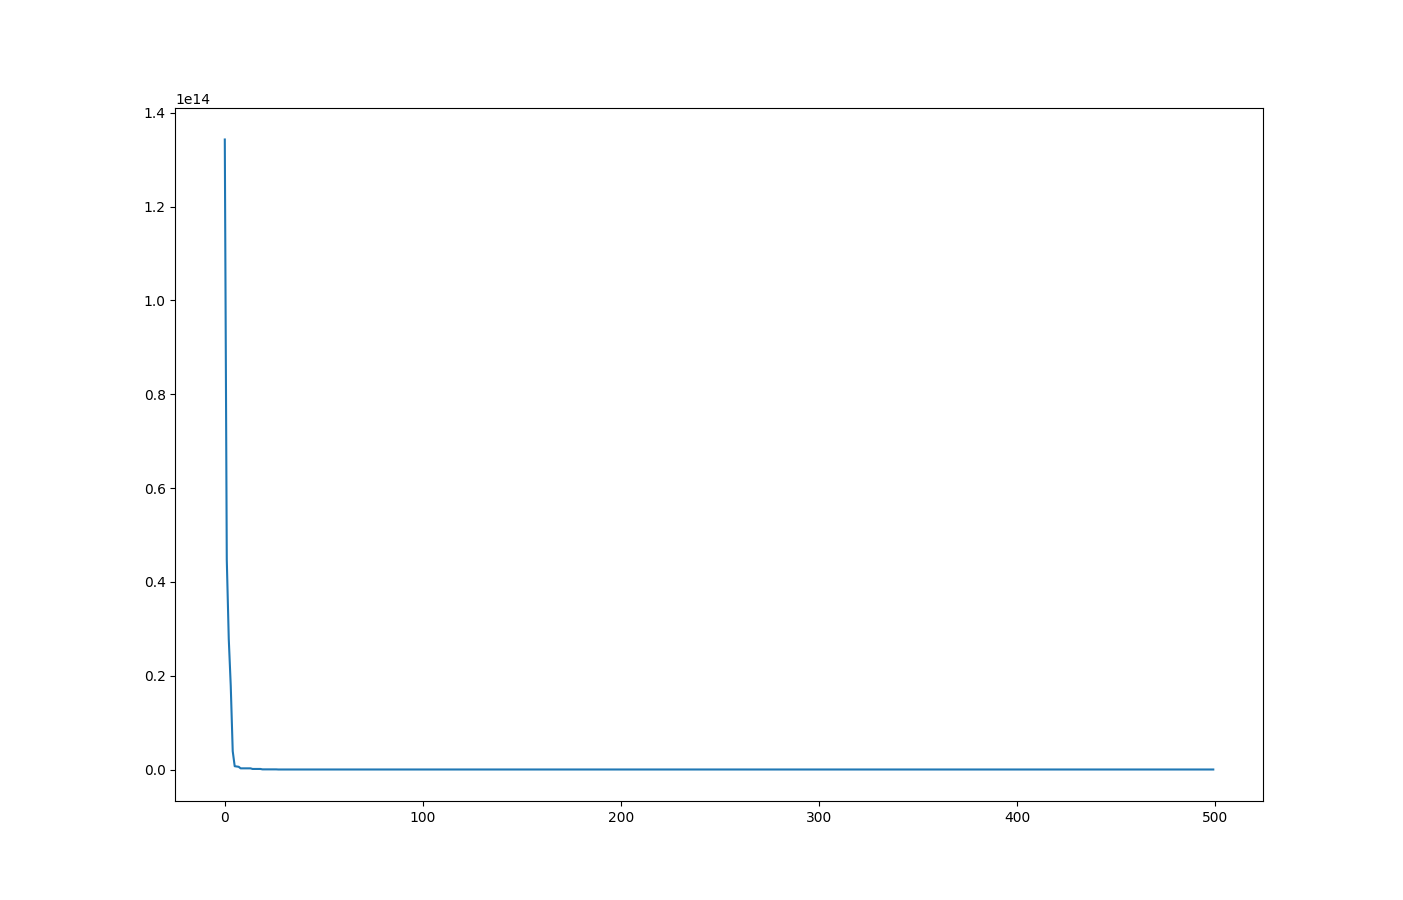
\includegraphics[width=23mm, height=20mm]{plots/bb4_naive.png} 
    & 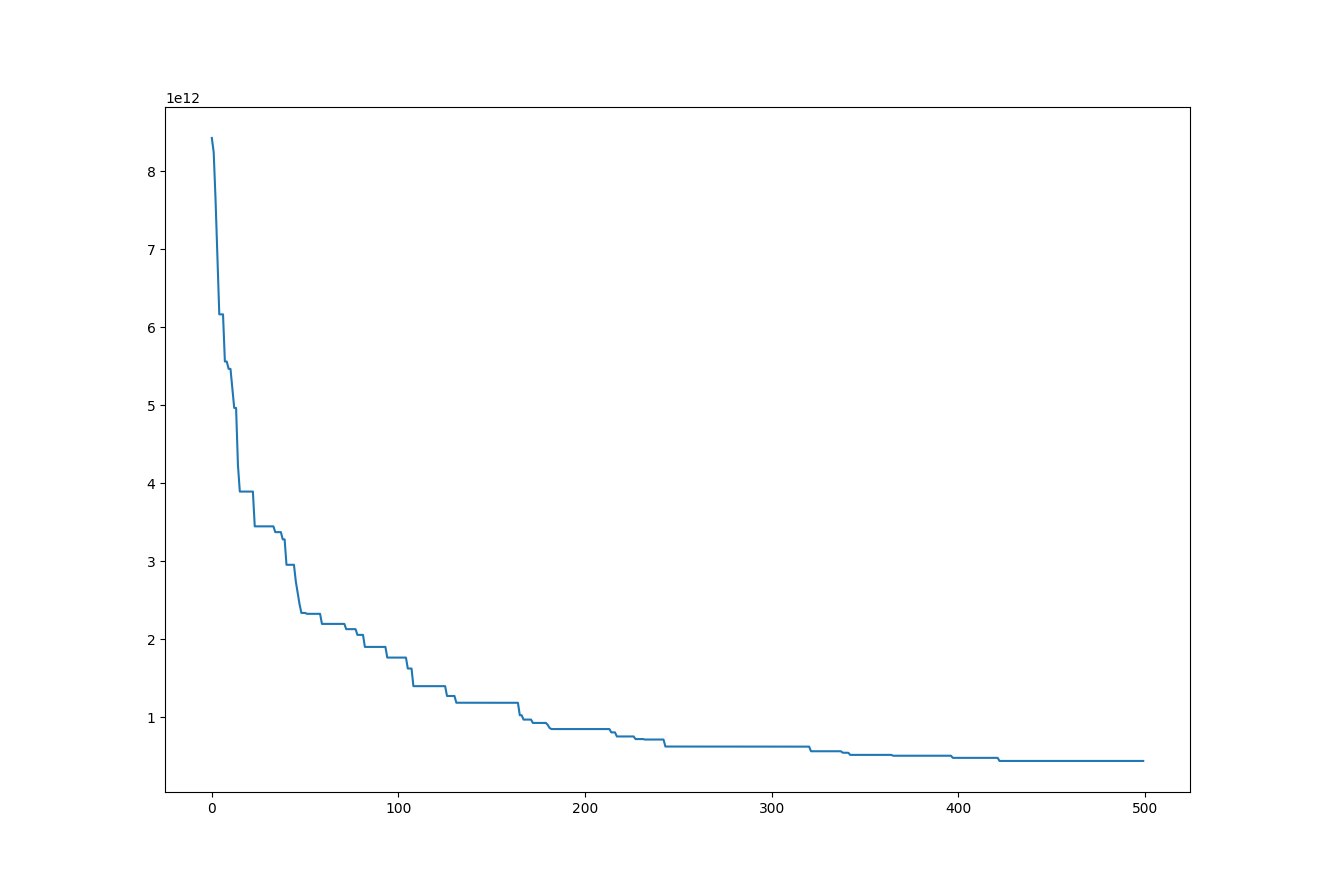
\includegraphics[width=23mm, height=20mm]{plots/bb4_ga_simple.png} 
    & 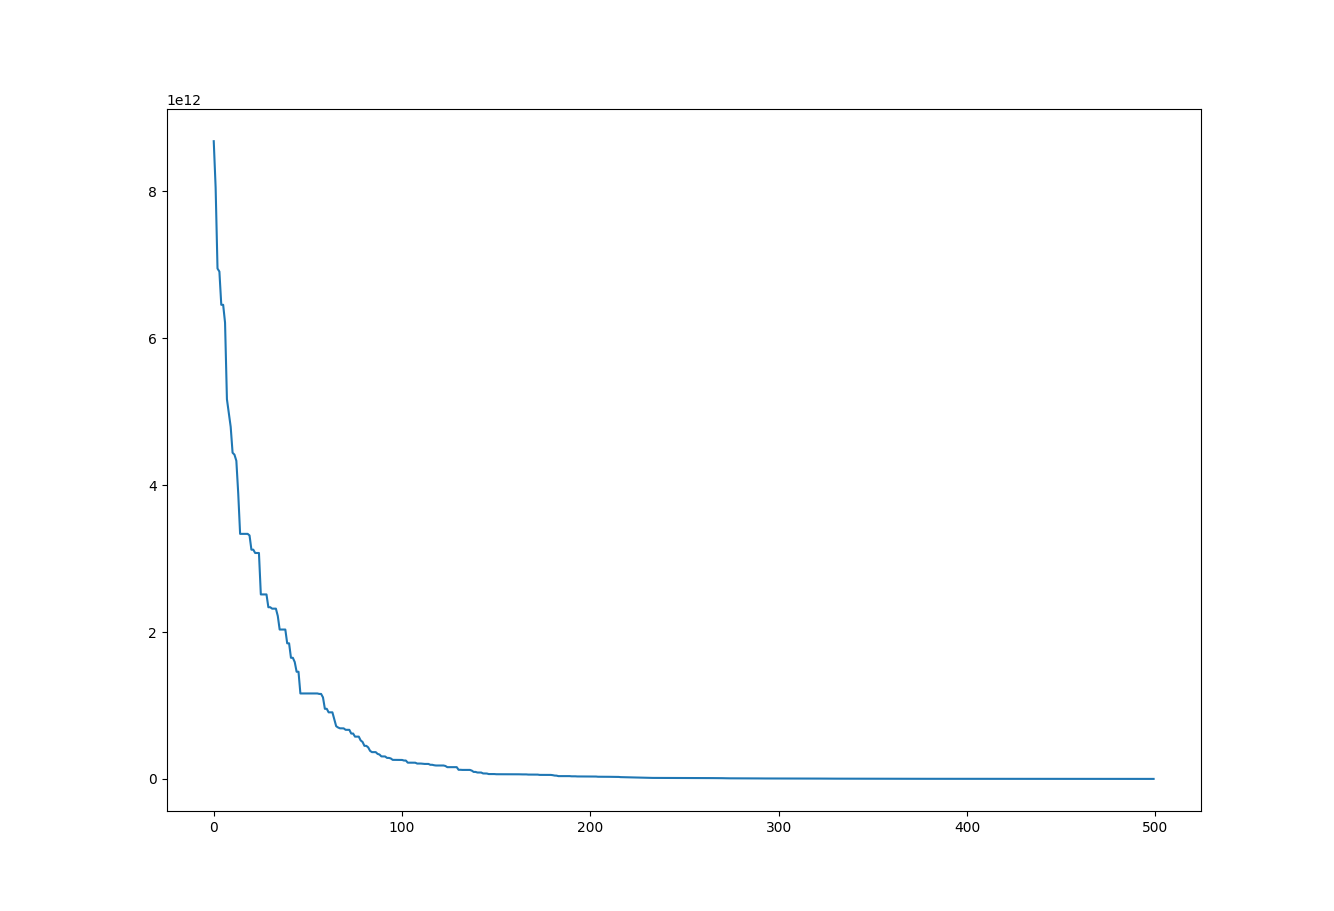
\includegraphics[width=23mm, height=20mm]{plots/bb4_ga_gray.png}
    & 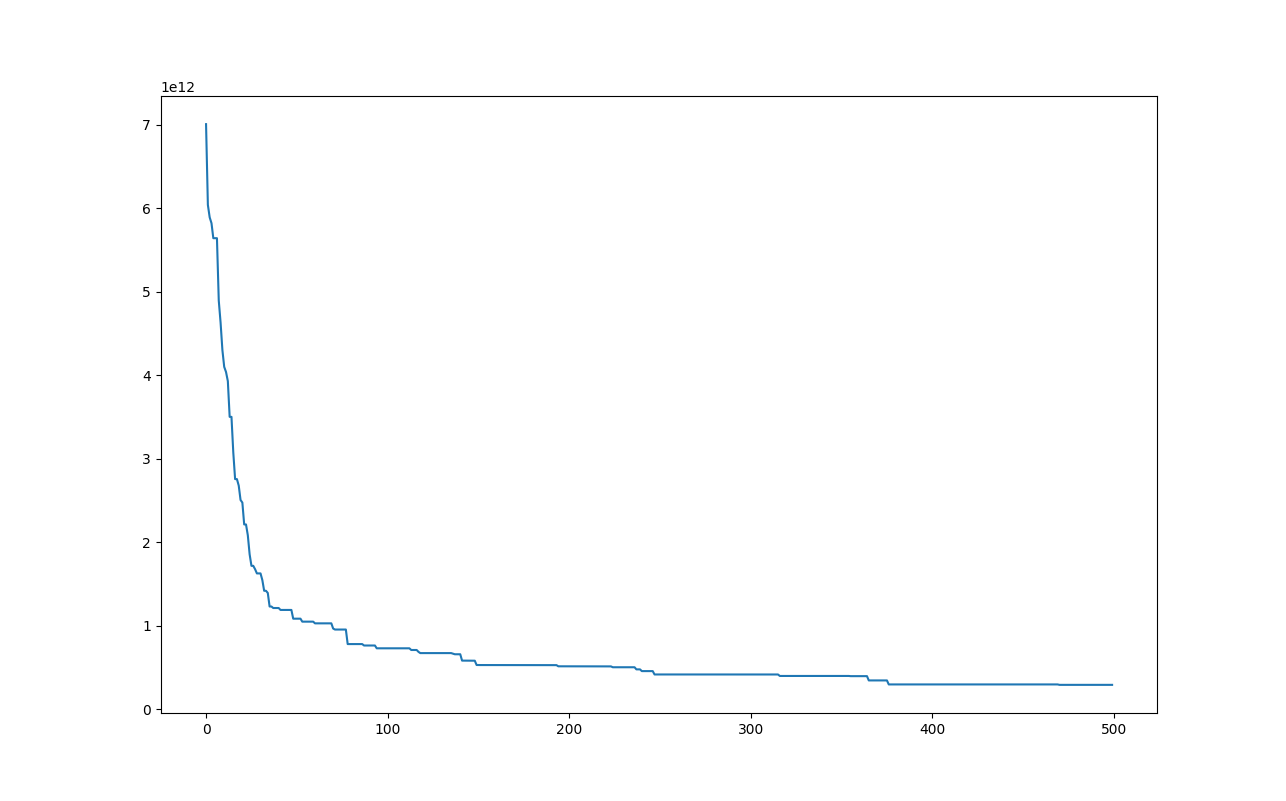
\includegraphics[width=23mm, height=20mm]{plots/bb4_ga_float.png} \\ \hline
      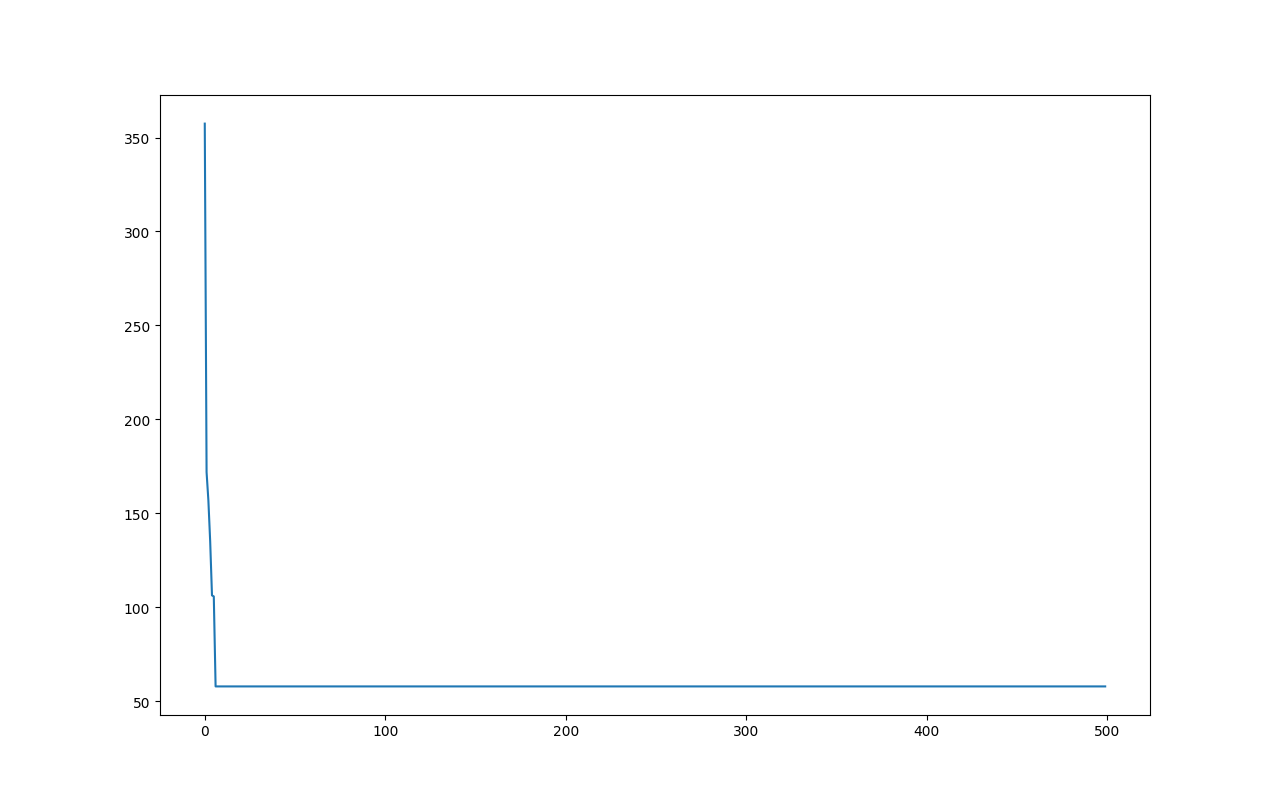
\includegraphics[width=23mm, height=20mm]{plots/bb4_hc.png} 
    & 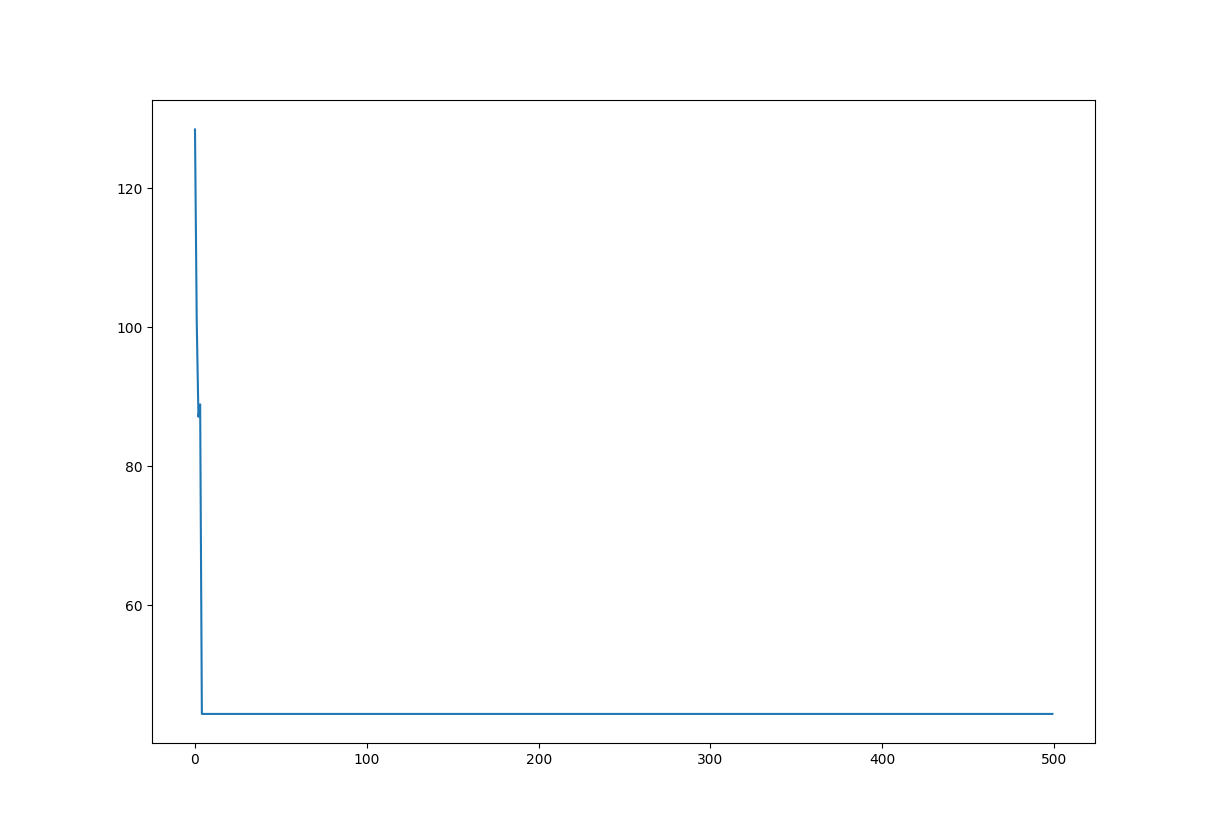
\includegraphics[width=23mm, height=20mm]{plots/bb4_hc_sa.png} 
    & 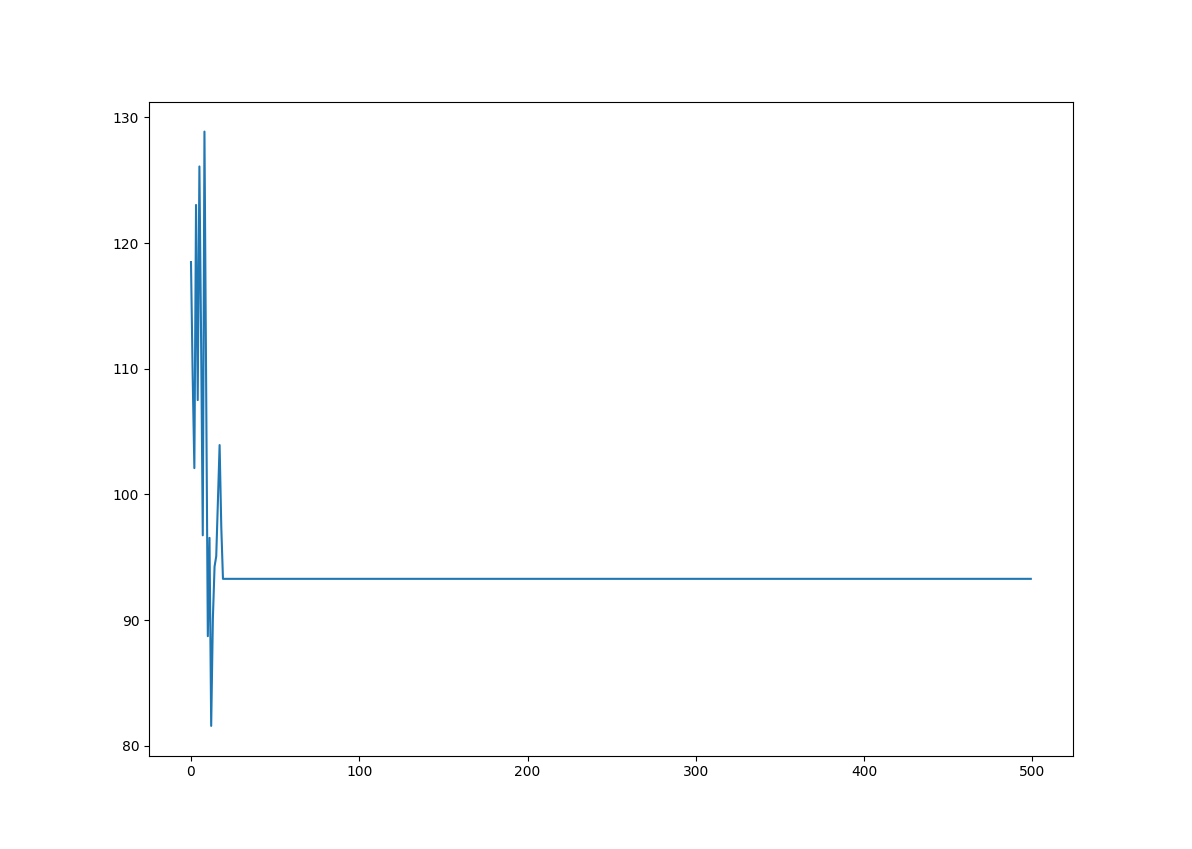
\includegraphics[width=23mm, height=20mm]{plots/bb4_hc_rs.png}
    & 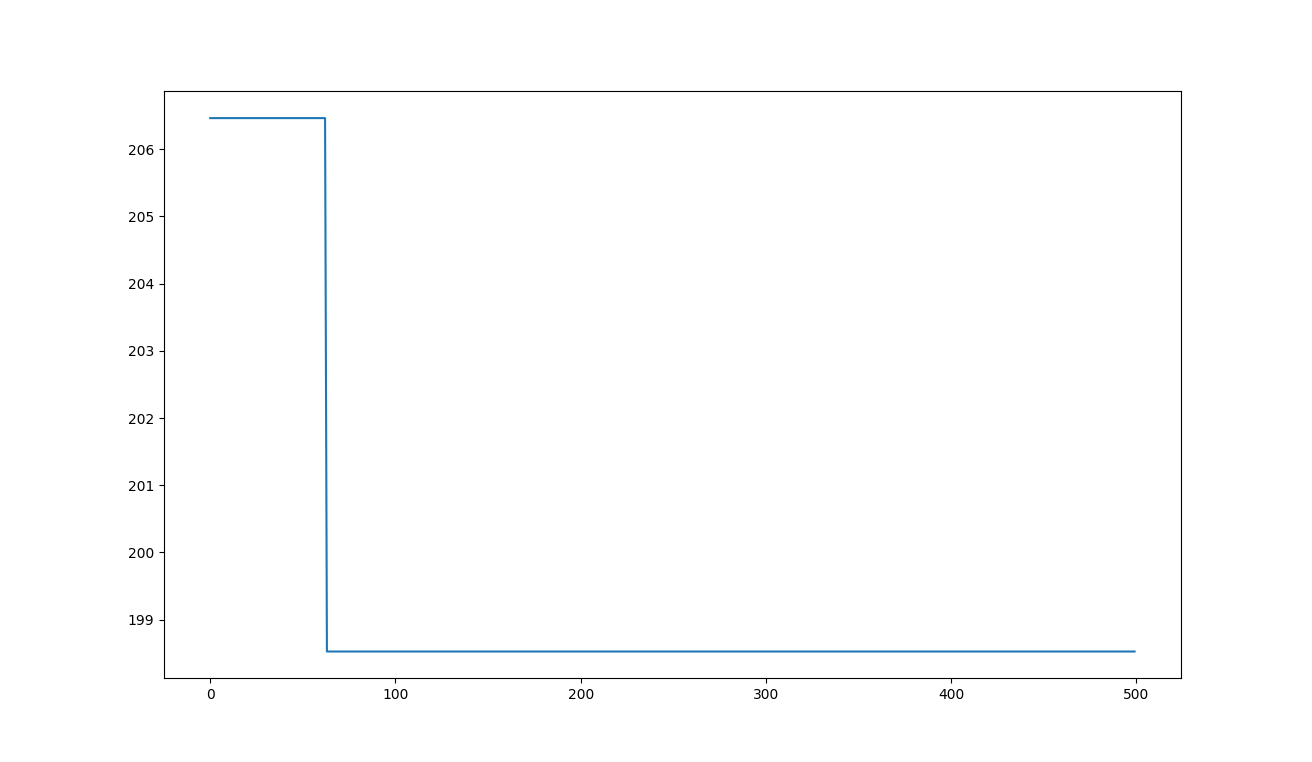
\includegraphics[width=23mm, height=20mm]{plots/bb4_sa.png} \\ \hline
    \end{tabular}
    \caption{Oben: Naives Verfahren, GA simple, GA gray, GA float \hspace{\textwidth}Unten: HC, HC steepest, HC random restart, simulated annealing}
    \end{figure}
    $\Rightarrow$ bestes Verfahren: ga-simple mit 100!
    \end{center}
\end{frame}

\begin{frame}{4 Auswertung BB5}
    \begin{center}
    \begin{figure}
    \begin{tabular}{|c|c|c|c|} 
      \hline
      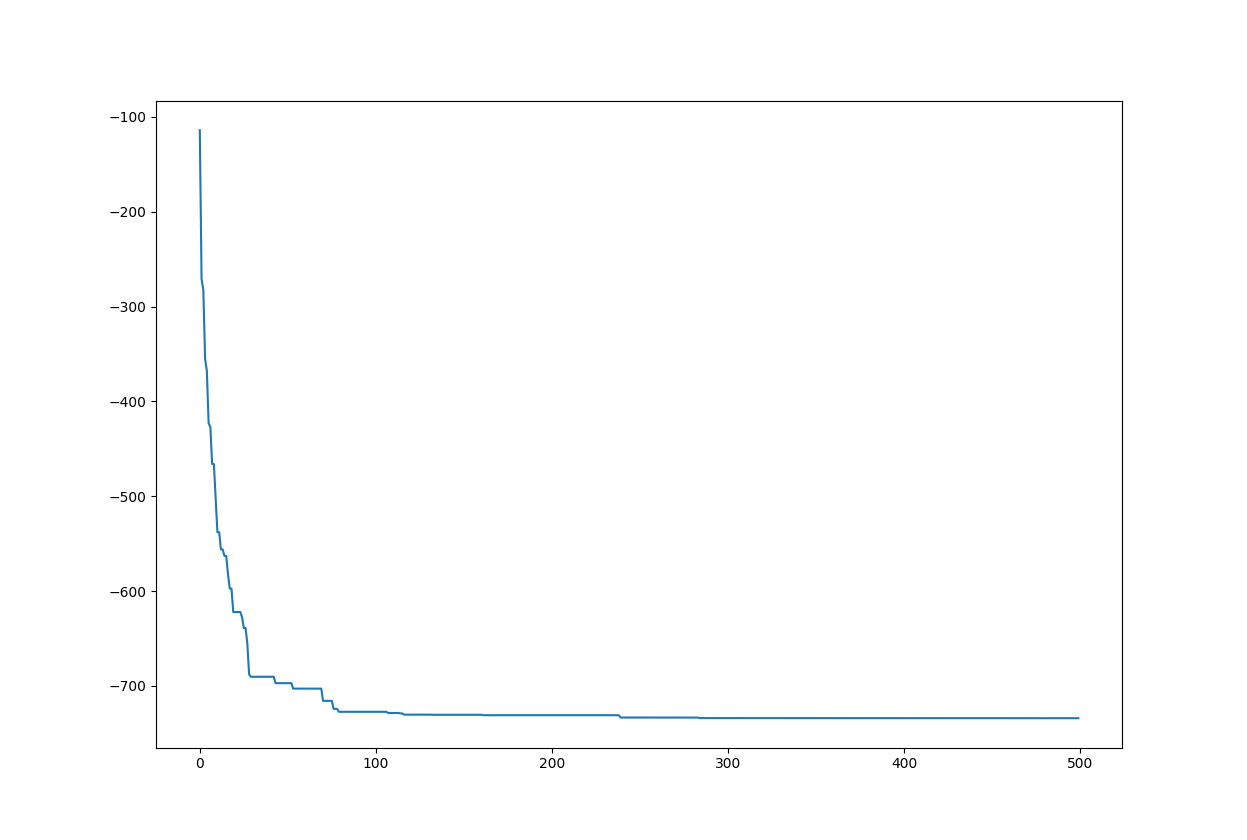
\includegraphics[width=23mm, height=20mm]{plots/bb5_naive.png} 
    & 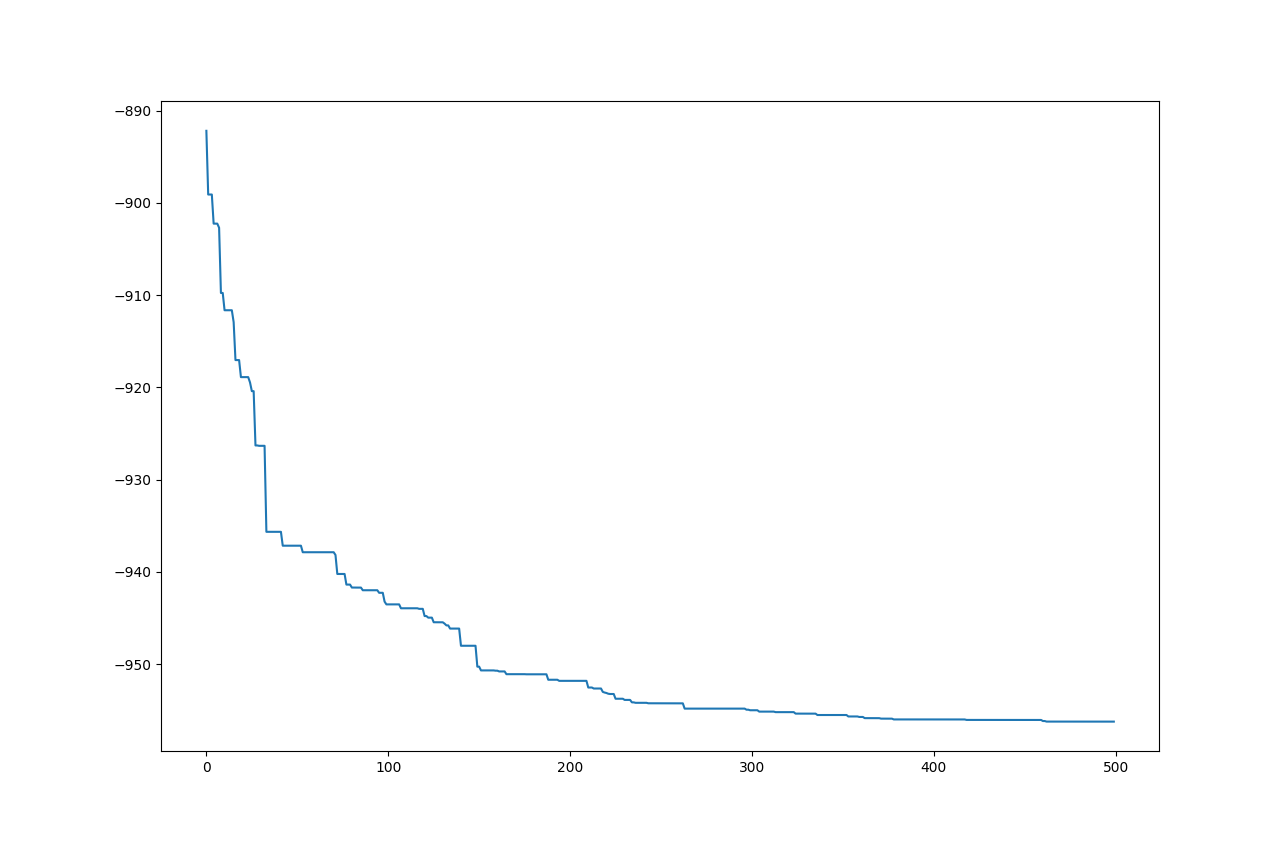
\includegraphics[width=23mm, height=20mm]{plots/bb5_ga_simple.png} 
    & 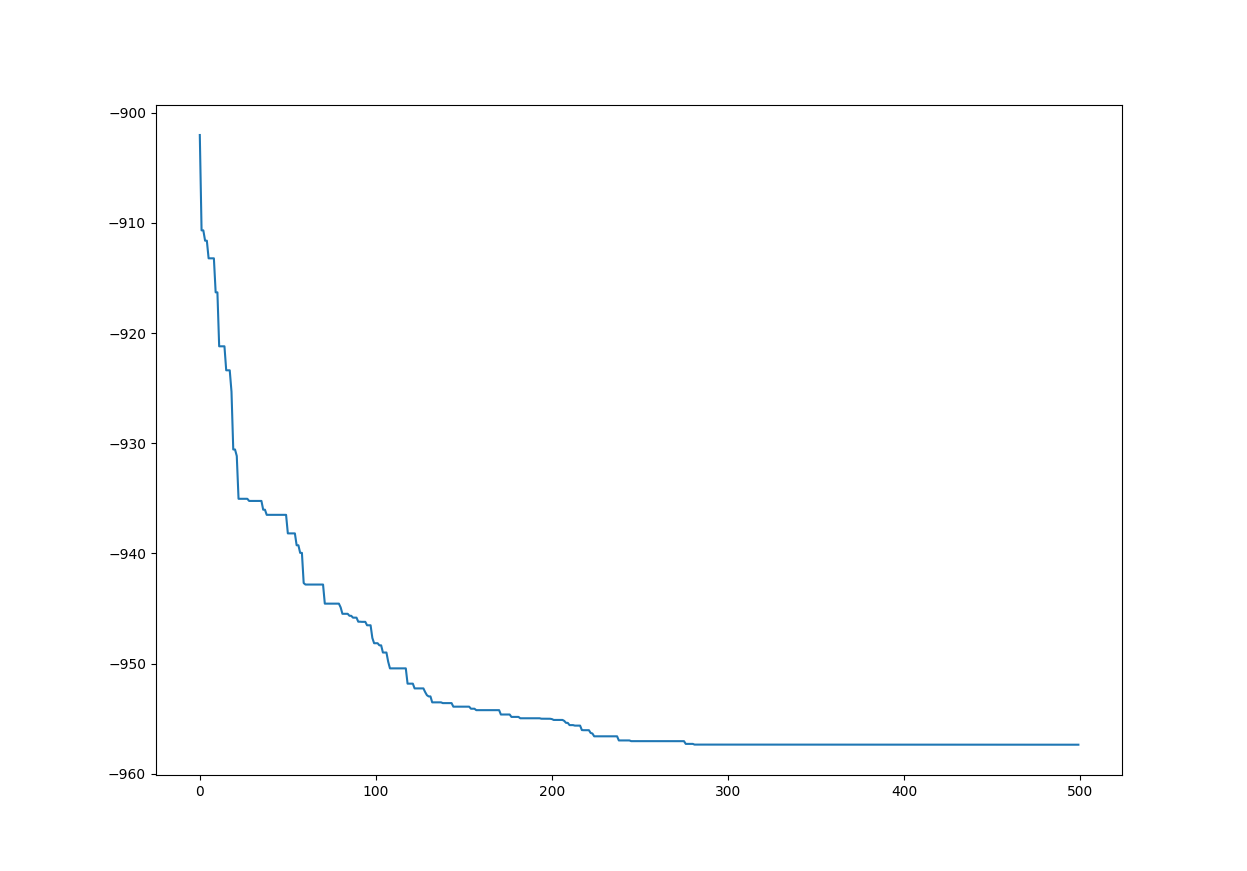
\includegraphics[width=23mm, height=20mm]{plots/bb5_ga_gray.png}
    & 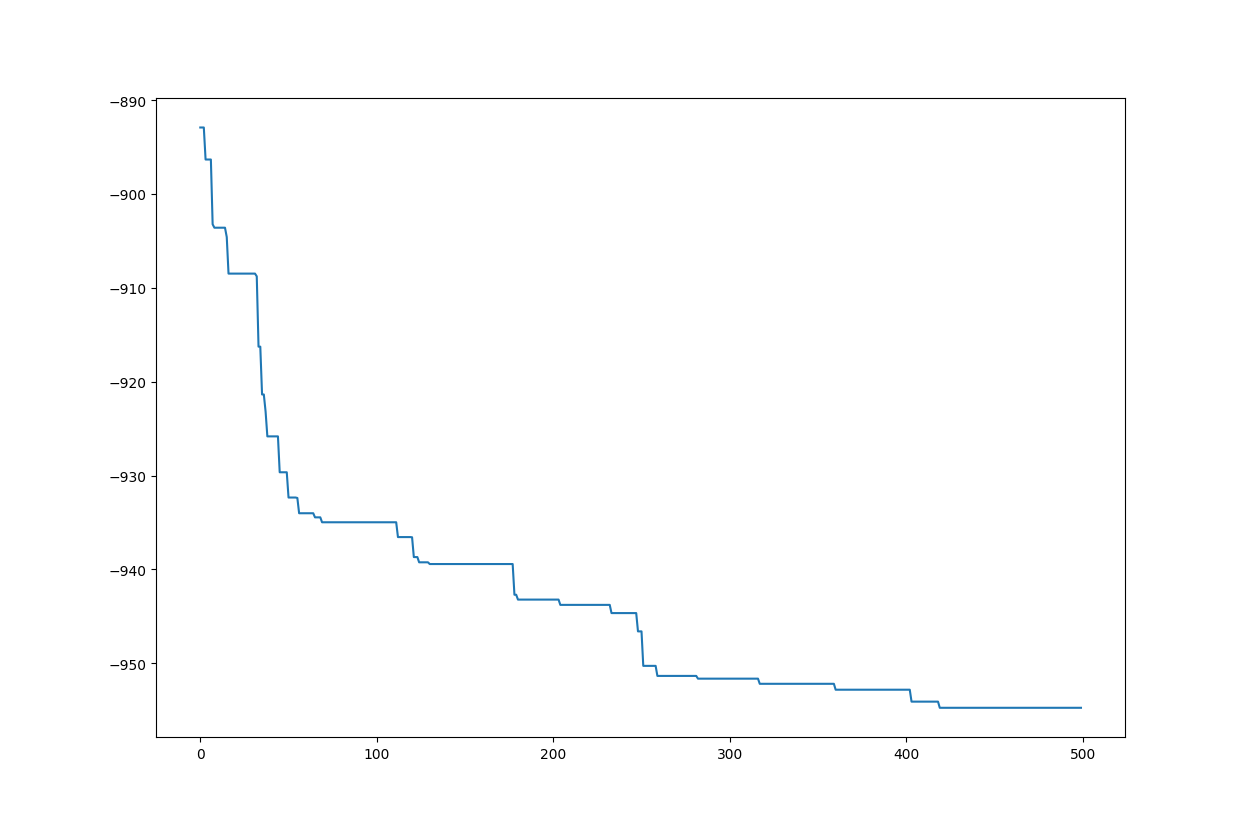
\includegraphics[width=23mm, height=20mm]{plots/bb5_ga_float.png} \\ \hline
      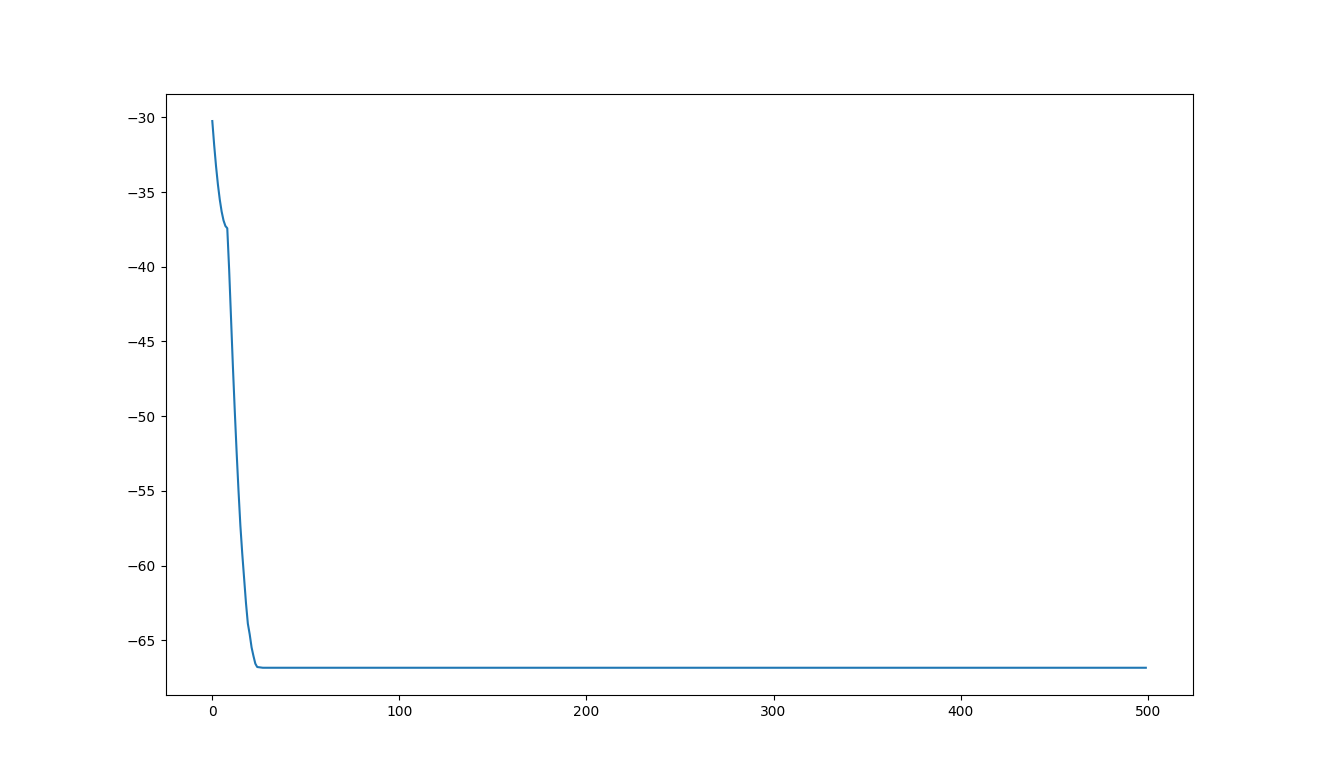
\includegraphics[width=23mm, height=20mm]{plots/bb5_hc.png} 
    & 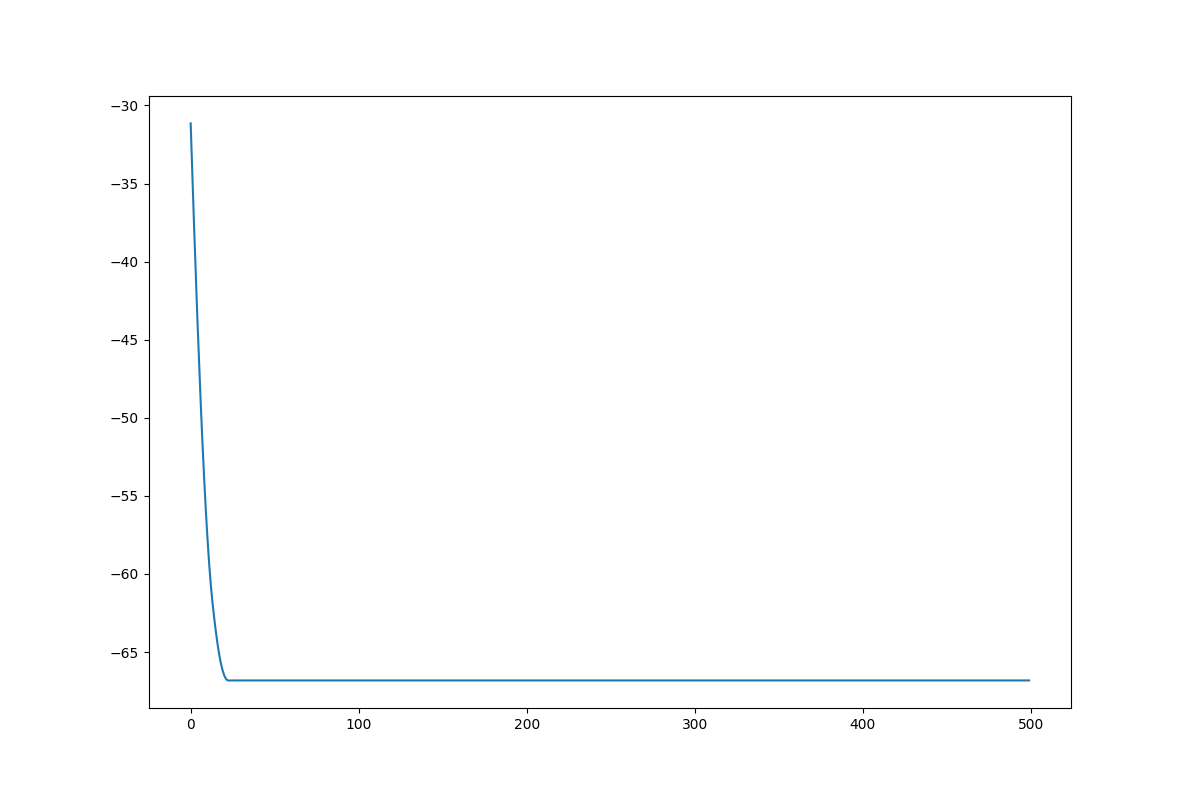
\includegraphics[width=23mm, height=20mm]{plots/bb5_hc_sa.png} 
    & 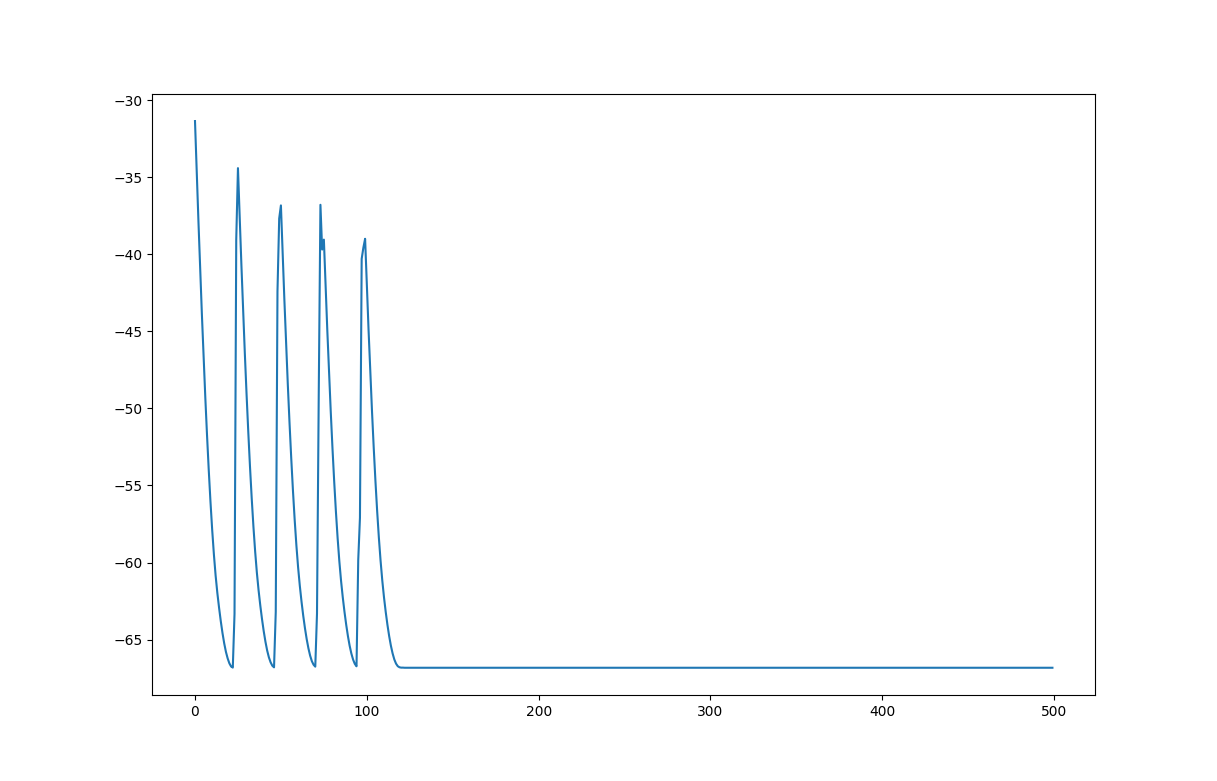
\includegraphics[width=23mm, height=20mm]{plots/bb5_hc_rs.png}
    & 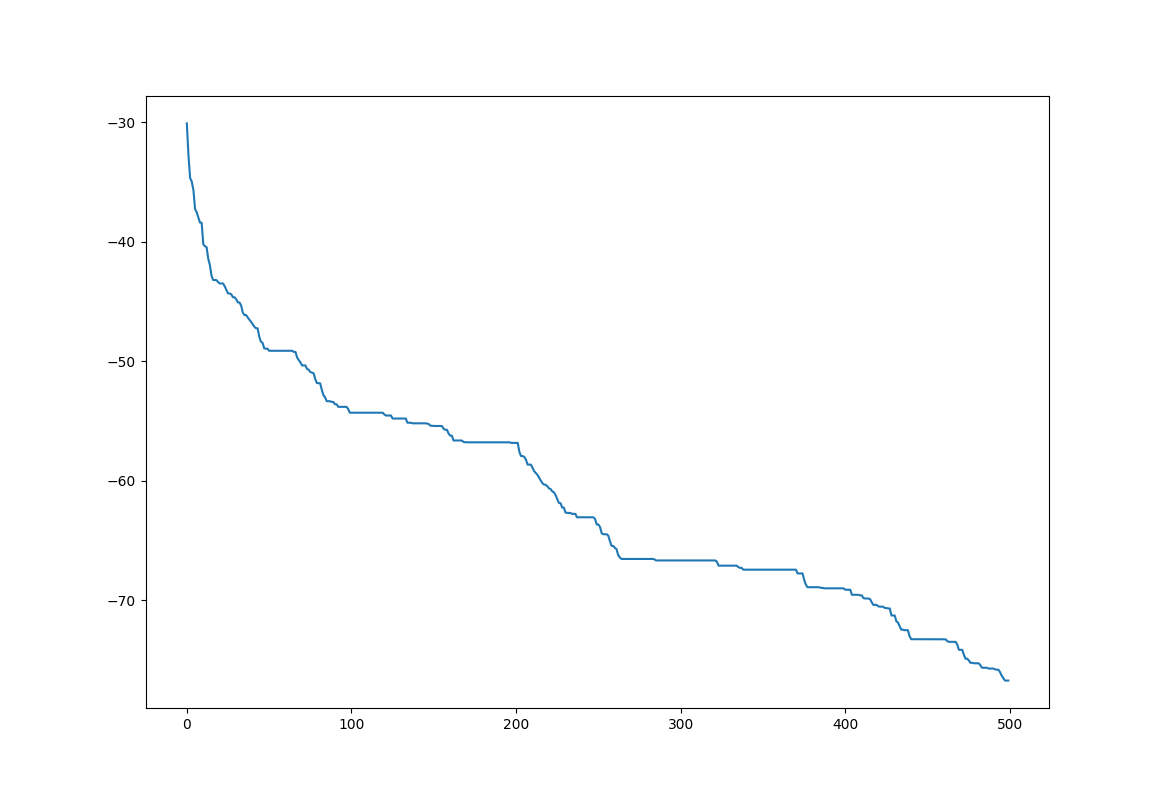
\includegraphics[width=23mm, height=20mm]{plots/bb5_sa.png} \\ \hline
    \end{tabular}
    \caption{Oben: Naives Verfahren, GA simple, GA gray, GA float \hspace{\textwidth}Unten: HC, HC steepest, HC random restart, simulated annealing}
    \end{figure}
    $\Rightarrow$ bestes Verfahren: ga-simple mit 100!
    \end{center}
\end{frame}

\begin{frame}{4 Auswertung}
Wie könnte man sich vorab für ein Verfahren entscheiden, wenn man nicht die Möglichkeit hat,
tausende Anfragen an die Blackbox zu stellen?
    \begin{itemize}
    \item 
    \end{itemize}
\end{frame}

\end{document}
% Local Variables:
% TeX-engine: xetex
% End:
